\chapterquote{%
Time and Space\dots It is not nature which imposes them upon us, it is we who impose them upon nature because we find them convenient.}%
{-- Henri Poincar\'e, \textit{The Value of Science} (1905)}

In this chapter\footnote{The present chapter was based on the articles \cite{dester2018} and \cite{dester2021part}.}, we include the spatial position of the nodes in the analysis.
%
Therefore, the transmission success probability $p_s$ can no longer be an arbitrary function of the traffic, because it needs to include the spatial positions into its model.
%
Thus, we need a more specific model for $p_s$, preferably one that entails analytical tractability.
%
In the following section, we propose a model inspired in Proposition~\ref{prop:PPP_ps} and other models adopted throughout the literature.

Another important concept we deal with in this chapter is the \textit{stability} of the queued packets. When a queue is not stable the number of queued packets tends to infinity \textit{almost surely} as time tends to infinity.
%
We are very interested in stable queues, because one of the important metrics, namely the delay, tends to infinity in unstable systems, and that is not desirable.

The additional notations used in this chapter are summarized in Table~\ref{tab:symbols}.
%
\begin{table}[hbt]
    \centering
    \caption{Notations and symbols used in this chapter}
    \label{tab:symbols}
    \setlength{\tabcolsep}{3pt}
    \begin{tabular}{l l}
      \hline
      \hline
      \textbf{Symbol} & \textbf{Definition/explanation} \\
      \hline
        $\alpha\in(2,\infty)$	& path loss exponent \\
        $\delta\in(0,1)$		& $\triangleq 2/\alpha$ \\
        $N \in \N^*$            & number of user classes \\
        $\cal{C}$				& $\triangleq \{1,2,\dots,N\}$, set of classes \\
        $n\in\cal{C}$			& refers to the $n$th user class \\
        $p_n\in(0,1)$			& medium access probability \\
      	$a_n\in(0,1)$			& packet arrival rate per time slot \\
        $\bm{a}\in(0,1)^N$		& $=(a_1,a_2,\dots,a_N)$ \\
        $p_{s,n}\in(0,1)$		& transmission success probability \\
        $\theta_n \in\R_+$		& SIR threshold for successful communication \\
        $\overline{R}_n\in\R_+$	& average transmission distance \\
        $D_n\in(1,\infty)$		& average packet transmission delay \\
        $\bm{D}\in(1,\infty)^N$ & $=(D_1,D_2,\dots,D_N)$ \\
        $P_n\in\R_+$			& transmission power \\
        $\bm{P}\in\R_+^N$ 		& $=(P_1,P_2,\dots,P_N)$ \\
        $\Phi_\TX^{(n)}$	    & Poisson point process for the transmitters \\
        $\lambda_n\in\R_+$		& density of $\Phi_\TX^{(n)}$ \\
        $\psi_n\in\R_+$			& $\triangleq 4\,\overline{R}_n^2 \,\theta_n^{\delta}     \,\pi\delta/\sin(\pi \delta)$ \\
        \hline
      \hline
    \end{tabular}
\end{table}

\newpage

% % % % % % % % % % % % % % % % % % % % % % % % % % 
% % % % % % % % % % % % % % % % % % % % % % % % % % 
\section{Multi-class High-mobility Bipolar Networks} \label{sec:N-class}

\subsection{Main Contributions}
The main contributions of the work presented in this section when compared to the literature, particularly the paper by Stamatiou and Haenggi \cite{stamatiou2010random}, are twofold.
%
Firstly, we have extended the analysis of stability (Definition~\ref{def:stability}) and delay in random-access wireless networks to the case of a network with an arbitrary number $N$ of user classes. As far as we know, this is the first time in the literature the stability region is found in closed form for a network with $N > 3$ different user classes sharing the same channel.
%
Secondly, we have expanded the analysis to show that the channel sharing mechanism in the investigated scenario can be seen as a process of partitioning a fixed and well-defined quantity into portions, each portion allotted to each user class, the size of which varying in accordance with the user class parameters.

More specifically, the novelty of the results on this section are summarized below:
\begin{itemize}[itemsep=3pt,parsep=3pt,topsep=3pt,partopsep=3pt]
    \item We propose a tractable scenario to study the performance and stability of a Poisson network with an arbitrary number $N$ of classes of users sharing the same channel;
    \item a simple and elegant expression relating mean delays, arrival rates, user densities, mean link distances, and bit rates of all $N$ classes is derived for the case of a stable network. This expression clearly shows that each class of user takes a well-defined portion of the available finite resource in the RF channel (Proposition~\ref{prop:identity_1});
    \item a closed form solution (Definition~\ref{def:closed_form}) to the fixed-point system of equations that determine the stationary transmission success probabilities for $N$ user classes is found;
    \item an intuitive equation is presented relating link quality, packet arrival rate, density of users, and stationary mean delay (Proposition 1);
    \item we prove the necessary and sufficient conditions that determine whether a given network is stable (Theorems \ref{TH:NEC_SUFF} and \ref{TH:STABILITY});
    \item we establish a simple necessary condition for stability that does not depend on the transmit powers (Corollary~\ref{cor:stab});
    \item the optimum transmit powers per user class that achieve the optimum stationary mean delays for each user class (Proposition~\ref{prop:opt}) are derived;
    \item the optimum packet arrival rates per user class that achieve the maximum channel throughput per unit of area (Proposition~\ref{prop:eps}) are derived;
    \item we conclude that depending on the channel and user classes, the best strategy to maximize channel throughput is to share the channel, instead of using one single class per channel.
\end{itemize}

% This section is organized as follows: Section \ref{sec:SysMod} describes the model used throughout the chapter and provides some important results from the literature to be used in the following sections;
% Section \ref{sec:N-users} presents the main results of the paper, i.e., necessary and sufficient conditions for stability when we have $N$ interacting user classes, and shows a simple expression for the stationary mean delay and the packet success probability; Section \ref{sec:application} applies the obtained results in two general scenarios: one scenario optimizes the transmission power of different user classes with different delay requirements sharing the same channel and the other optimizes the throughput per unit of area; Section \ref{sec:conclusion} concludes the paper.


\subsection{System Model}

We consider a stationary high-mobility Poisson network with density $\lambda$ on $\R^2$ and with $N$ classes of users that share the same radio frequency channel as defined in the general network model of Chapter~\ref{cap:P2_00}.
%
Time is slotted, $\T=\N$, and for each time slot $t \in \T$ and each user class $n \in \cal{C} \triangleq \{1,2,\dots,N\}$, we have a homogeneous Poisson point process (PPP) denoted by $\Phi_\TX^{(n)}(t)\stackrel{*}{=} \{ X_{i\,n}(t) \}_{i\in\N}$ of density $\lambda_n$ on $\R^2$, which represents the position of the sources. These PPPs are independent from each other and from the past.
%
Furthermore,
\begin{align*}
    \lambda = \sum_{n\in\cal{C}} \lambda_n,
    \quad\text{then,}\quad
    \Phi_\TX(t) = \sum_{n\in\cal{C}} \Phi_\TX^{(n)}(t) \quad\text{for every $t\in\T$}.
\end{align*}

\begin{remark}
    Using the general network model of Chapter~\ref{cap:P2_00}, the set of transmitters $\cal{N}_\TX = \N\times\cal{C}$. Thus, each transmitter should be indexed by a number and a class. However, for ease of notation and since the network is stationary across the users within a class, we shall omit the number and only refer to the class for parameters and metrics.
    %
    For example, the transmission success probability $p_{s,n}$ refers to $p_{s,\N\times\{n\}}$, i.e., it refers to the set of all users from $n$th class (or a typical user of that class).
\end{remark}

\begin{figure}[H]
    \centering
    \if\printfig1
        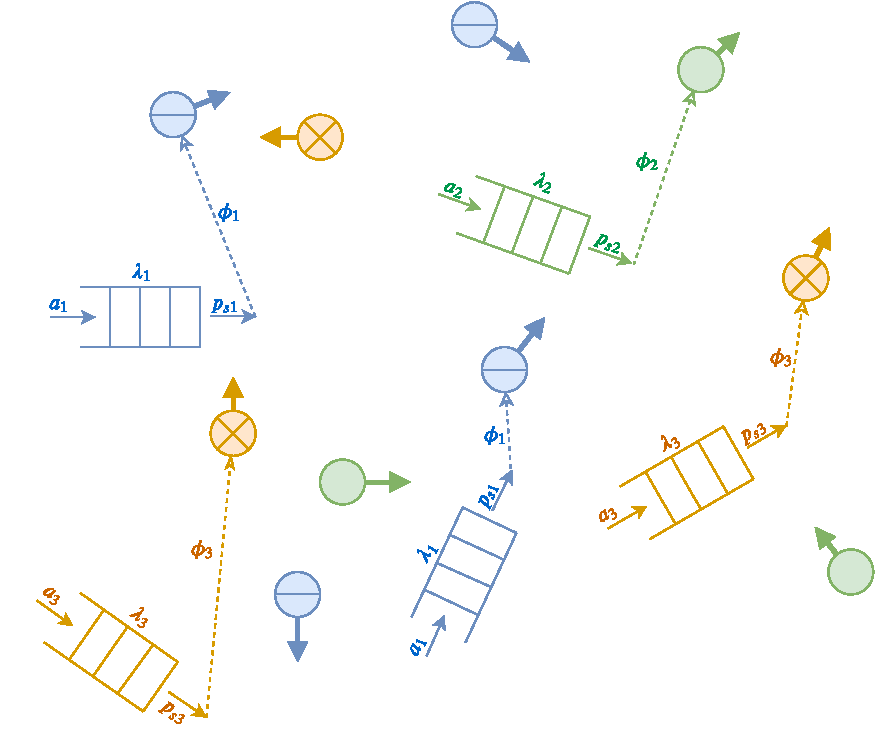
\includegraphics[width=0.8\textwidth]{Figures/Ch7_BipolarQueuedNetwork.pdf}
    \else
        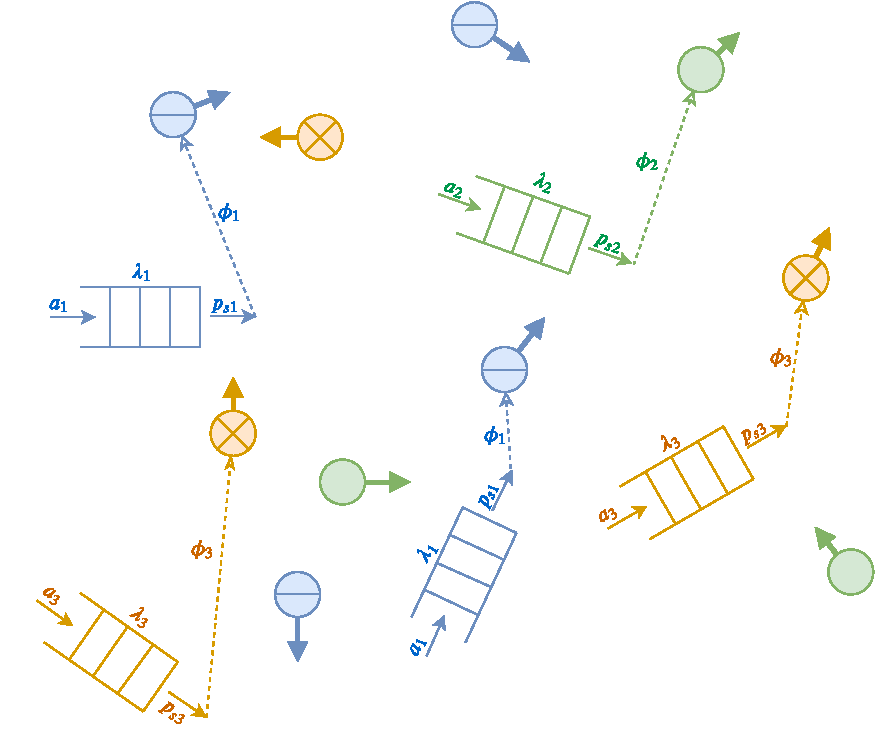
\includegraphics[draft,width=0.8\textwidth]{Figures/Ch7_BipolarQueuedNetwork.pdf}
    \fi
    \caption{Example of a bipolar high-mobility random network with $N=3$ user classes (one for each color). The queues represent the transmitters, and the potential receivers are represented by circular shapes of the corresponding color. The purpose of the arrows is to remember that the nodes are moving. Each transmitter communicates with the closest potential receiver, as it is shown by the dashed lines. Unconnected circles represent inactive receivers. The quantities $\lambda$, $a$, $p_s$ and $\phi$ are related to density of users, rate of arrival of packets, rate of service of packets and link quality, respectively.}
    \label{fig:BipolarNetwork}
\end{figure}

Each transmitter of user class $n$ transmits with power $P_n$ constant over time, and the transmitted signal is subjected to Rayleigh short-term fading and power law path loss function $\ell(r) = r^{-\alpha}, r>0$, where $\alpha>2$ is the path loss exponent.

% For each time slot the position $X_{i\,n}(t)$ of the $i$th transmitter is reallocated following the high-mobility random walk model \cite{baccelli2010stochastic}.
%
% The $i$th transmitter of user class $n$ communicates with a receiver located at $Y_{i\,n}(t)$. Thus, the distance between the $i$th transmitter of class $n$ and its destination is given by $R_{i\,n}(t) = || X_{i\,n}(t) - Y_{i\,n}(t) ||$.
%
We further assume that each transmitter is associated with a ``son'' PPP that models the locations of its potential receivers. The receiver associated with the $i$th transmitter of class $n$ is chosen as the closest point in the respective son PPP as illustrated in Figure~\ref{fig:BipolarNetwork}.

As a consequence, the link distances $\{ R_{i\,n}(t) \}_t$ are iid Rayleigh random variables\footnote{The iid random variables for the link separation distance are of grave importance for the theoretical model. Otherwise, there would exist unstable queues and, consequently, the queueing network would be unstable.} \cite[Eq.~(2.35)]{kingman1992poisson}.
%
Rayleigh distributed link separation distance has been used in several other works investigating similar scenarios (see \cite{haenggi2013diversity}).
%
We denote the mean transmission distance $\E[R_{i\,n}(t)]$ simply by $\overline{R}_n$ because we have stationarity across time and across users of a given class. Then, the density of $R_{i\,n}$ can be expressed as
\begin{align*}
    f_{R_n}(r) = \frac{\pi\,r}{2 \overline{R}_n^2} \exp\!\left[ - \frac{\pi\,r^2}{4\overline{R}_n^2}\right], \qquad r\in\R_+.
\end{align*}

The occupation of the buffer at each transmitter is represented by its queue length $\{ Q_{i\,n}(t) \}_t$ of infinite capacity.
%
The packet arrival probability at each queue is denoted by $a_n$ and the medium access probability by $p_n$.
%
Within each slot, the first event to take place for each transmitter with a non-empty queue is the medium access decision with probability $p_n$. If it is granted access and the signal to interference ratio (SIR) %\footnote{We assume thermal noise is negligible; refer to \cite{haenggi2012stochastic} for further details.}
is greater than a threshold $\theta_n>0$, a packet is successfully transmitted and leaves the queue. Then, we have the arrival of the next packet with probability $a_n$. The last event to take place is the displacement of the transmitters and destinations.

The queue lengths of the $i$th transmitter, user class $n$ are Markov chains represented by
\begin{equation*}
	Q_{i\,n}(t+1) = (Q_{i\,n}(t) - B_{i\,n}(t))_+ + E_{i\,n}(t), \quad t \in \N,
\end{equation*}
where $(\cdot)_+ \triangleq \max\{\cdot,0\}$, $\{E_{i\,n}(t)\}_t$ are iid Bernoulli random variables of parameter $a_n$, i.e., $E_{i\,n}(t)\sim\mathscr{B}(a_n)$ and represents the arrival process,
$
	B_{i\,n}(t) = e_{i\,n}(t)\,\ind\{\text{SIR}_{i\,n}(t)>\theta_{n}\}
$
represents the departure process, where $\{e_{i\,n}(t)\}_t$ are iid Bernoulli random variables of parameter $p_n$, i.e., $e_{i\,n}(t)\sim\mathscr{B}(p_n)$, and the constant $\theta_n > 0$ represents the SIR threshold for successful communication.

\begin{remark}
        In view of the model of Chapter~\ref{cap:P2_00}, we have that the arrival point process $A_{i\,(n)}$ is a Bernoulli point process of parameter $a_n$, the access point process $T_{i\,(n)}$ is a Bernoulli point process of parameter $p_n$ and the transmissions times $T_{i\,(n)}^*$ is a thinning of $T_{i\,(n)}$ conditioned to the corresponding queue being non-empty, and the success probability model $\mathscr{S}(f) = \ind\{f(0) > 1\}$, where $f(t') = \SIR_{i\,n}(t-t')/\theta_n$.
\end{remark}

% % % % % % % % % % % % % % % % % % % % % % % % % % % % % %
\subsection{Analysis and Results}
\label{ssec:N-users}

From the stationarity across users of a class and ergodicity regarding time (if the system is stable), the transmission success probability $p_{s,n}$ is the limiting probability of a successful transmission from a typical user of class $n$, i.e., $$p_{s,n} = \lim_{t\to\infty} \P(\mathrm{SIR}_{i,n}(t) > \theta_n).$$

\begin{note}
    Remember that, \textit{à priori}, we do not need to take $t\to\infty$, any $t$ would suffice in an ergodic process.
    %
    However, as discussed in Section~\ref{sec:poisson_network} we would have to start the system at $-\infty$ or start the system distributed according to the stationary distribution.
\end{note}

The stationary mean delay $D_n$ to transmit packets of class $n$ is defined as the limiting ($t\to\infty$) expected time a packet spends in the buffer and the server.
%
See Theorem~\ref{th:little}.
% For each time slot and for each class we have an independent homogeneous PPP, which is stationary and isotropic (invariant to translation and rotation, respectively).

% The following results from the literature are used in many proofs throughout the chapter. In a wireless network, let us assume that \textit{(i)} the separation distance between a given pair TX - RX is equal to $r$, \textit{(ii)} the positions of the interferers (users who will transmit packets in a given time slot) follow a PPP of density $\lambda_\mathrm{eff}$, and \textit{(iii)} every transmitter has the same transmit power. Then, the probability of a successful transmission between TX and RX is given by \cite[Sec.~III.A]{haenggi2009stochastic}
% \begin{align}
% 	\P(\mathrm{SIR} > \theta) &= \E[\euler^{-\theta r^\alpha I}] \nonumber\\
%     	&= \exp\left( - \pi\,\Gamma(1+\delta) \Gamma(1-\delta)\,\theta^{\delta}\,r^2\,\lambda_\mathrm{eff} \right),
% \end{align}
% where $\delta \triangleq 2/\alpha$ and $I \triangleq \sum_{X\in\Phi} ||X||^{-\alpha}$ is the interference received by RX normalized by the transmit power and $\Phi$ is a PPP of density $\lambda_\mathrm{eff}$, which is the effective density of active sources.
%

% As described in the previous section, we consider a network with $N$ classes of users.
%
The following proposition presents the stationary success probability and mean delay when transmitting a packet in a stable network. The results that guarantee stability are presented later in the sequence, in Theorem~\ref{TH:NEC_SUFF}.

\begin{proposition} \label{prop:psk}
	If the network is stable, then the stationary success probability and mean delay for a typical user of class $n \in \cal{C}$ are given by
	\begin{align}
    	p_{s,n} &= \left( 1 + \dfrac{\psi_n}{P_n^\delta}\, 
        \dfrac{\sum_j P_j^\delta\,a_j\lambda_j}
        {1 - \sum_j \psi_j\,a_j\lambda_j} \right)^{-1},\label{eq:psn}\\ 
        D_n &= \dfrac{1 - a_n}{p_n\,p_{s,n} - a_n},	\label{eq:Dn}
    \end{align}
    where the sums are taken over the set of user classes $\cal{C}$, ${\delta \triangleq 2/\alpha}$, and 
    \begin{equation}\label{eq:DefPhi}
        \psi_n
            \triangleq 4\,\Gamma(1+\delta) \Gamma(1-\delta) \overline{R}_n^2 \theta_n^\delta
            = 4\,\overline{R}_n^2\,\theta_n^{\delta}\, \frac{\pi\delta}{\sin(\pi \delta)}.
    \end{equation}
\end{proposition}

\begin{proof}
    First, we need to calculate the transmission success probability for a given traffic and a given link distance.
    %
    Using the reasoning of Proposition~\ref{prop:PPP_ps} for the case of several classes of users, we have
    \begin{align} \label{eq:P_SIR}
    	\P(\text{SIR}_{i\,n}(t)>\theta_n \mid R_{i\,n}) &= \E\!\left[\exp\left(-\frac{\theta\,R_{i\,n}^\alpha}{P_n} \sum_{k\in\cal{C}} P_k\,I_k\right)\right]\nonumber\\
        	&= \prod_{k\in\cal{C}} \E\!\left[\exp\left(-\theta\,R_{i\,n}^\alpha\frac{P_k}{P_n} I_k\right)\right] \nonumber\\
            &= \prod_{k\in\cal{C}} \exp\!\left( - \pi R_{i\,n}^2\, \theta^{\delta}\,\frac{\pi\delta}{\sin(\pi\delta)} \frac{P_k^\delta}{P_n^\delta}\lambda_\mathrm{eff}^{(k)}(t)\right) \nonumber\\
        	&= \exp\!\left( - \pi R_{i\,n}^2\,\theta^{\delta}\,\frac{\pi\delta}{\sin(\pi\delta)} \,\sum_{k\in\cal{C}}\frac{P_k^\delta}{P_n^\delta}\lambda_\mathrm{eff}^{(k)}(t)\right),
    \end{align}
    where $I_n$ is the interference from the $n$th class normalized by the transmit power, and $\lambda_{\mathrm{eff}}^{(n)}$ is the density of the thinned Poisson point process $\Phi_\TX^{(n)}$ by the nodes that are transmitting.
    %
    It is assumed that $\{I_n\}_{n \in \cal{C}}$ is iid.

    As $t\to\infty$, the effective PPP density of active sources $\lambda_\mathrm{eff}^{(n)}$ for each user class $n\in\cal{C}$ converges (by hypothesis) to $\lambda_n\,p_n\,\rho_n$, where $\rho_n = a_n/(p_n\,p_{s,n})$ is the load of the queue (or the probability of having a non-empty queue), which is the ratio between the arrival rate and the service rate of packets. Thus, $\lambda_\mathrm{eff}^{(n)} = \lambda_n\,a_n/p_{s,n}$.

    Then, to calculate the transmission success probability $p_{s,n}$, we use \eqref{eq:P_SIR}. Thus, by deconditioning the transmission success probability on $R_{i\,n}$, we take into account that $R_{i\,n}$ is Rayleigh distributed, that is
    \begin{align} \label{eq:aux_psk}
    	p_{s,n} &= \lim_{t\to\infty}\P(\text{SIR}_{i\,n}(t)>\theta_n) \nonumber\\
        	&= \int_0^\infty \lim_{t\to\infty} \P(\text{SIR}_{i\,n}(t)>\theta_n
            	\mid R_{i\,n}(t) = r)\,f_{R_n}(r)\,\mathrm{d}r \nonumber\\
            &= \int_0^\infty \frac{\pi r}{2 \overline{R}_n^2} \exp\!\left[ - \frac{\pi\,r^2}{4\overline{R}_n^2} \left(1+\psi_n\sum_{k\in\cal{C}}\frac{P_k^\delta}{P_n^\delta}\lambda_\mathrm{eff}^{(k)}\right)\right]\mathrm{d}r \nonumber\\
            &= \left( 1 + \dfrac{\psi_n}{P_n^\delta}
      			\sum_{k\in\cal{C}} P_k^\delta \dfrac{a_k\lambda_k}{p_{s,k}} \right)^{-1}.
    \end{align}
    This expression can be rearranged as
    \begin{equation} \label{eq:psk_equivalence}
    	\dfrac{P_n^\delta}{\psi_n} \left( \dfrac{1-p_{s,n}}{p_{s,n}}\right) = 
        \sum_{k\in\cal{C}} P_k^\delta \dfrac{a_k\lambda_k}{p_{s,k}}.
    \end{equation}
    Note that the right-hand side of \eqref{eq:psk_equivalence} does not depend on $n$. Then, for all $j\in\cal{C}$, we have%
    \begin{equation} \label{eq:Pi_Pk}
    	\dfrac{P_j^\delta}{\psi_j} \left( \dfrac{1-p_{s,j}}{p_{s,j}}\right) = 
        \dfrac{P_n^\delta}{\psi_n} \left( \dfrac{1-p_{s,n}}{p_{s,n}}\right).
    \end{equation}
    For each $j$, we can solve the above equation for $p_{s,j}$ and plug it into the sum of \eqref{eq:aux_psk}. Then, we can solve it for $p_{s,n}$, which ends the proof for the $p_{s,n}$.
    
    The buffer (plus server) is a discrete time Geo/Geo/1 queue (Definition~\ref{def:geo/geo/1}) at stationary \cite{stamatiou2010random} and the equation for the delay $D_n$ comes from Theorem~\ref{th:geo/geo/1}.
\end{proof}

The following theorem shows the conditions for which the network is stable, i.e., it presents the region formed by all arrival rates $\bm{a}$ that make the system stable.

\begin{theorem} \label{TH:NEC_SUFF}
	A necessary and sufficient condition for the system network to be stable is that $\bm{a} \in \bigcup_{\nu\in\cal{V}} \cal{E}_\nu$, where $\cal{V}$ is the space of all bijective functions from $\cal{C}$ to $\cal{C}$ and $\cal{E}_\nu$ is defined below with the convention $\sum_{k=1}^0 \cdot = 0$.
	\begin{align} \label{eq:stab_long}
    	\cal{E}_{\nu} \triangleq \Bigg\{ \bm{a} \in [0,1)^N \Bigm\vert~ 
    	& 0 \le 
        \dfrac{\psi_{\nu(n)}}{P_{\nu(n)}^\delta}\dfrac{a_{\nu(n)}}{p_{\nu(n)}-a_{\nu(n)}} \nonumber\\
        & < \dfrac{ 1 - \sum_{k=1}^{n-1} \psi_{\nu(k)} a_{\nu(k)} \lambda_{\nu(k)} }
        {\sum_{k=1}^{n-1} P_{\nu(k)}^{\delta} a_{\nu(k)}\lambda_{\nu(k)} +
        \sum_{k=n}^N P_{\nu(k)}^\delta p_{\nu(k)}\lambda_{\nu(k)}},
        \quad n \in \cal{C} \Bigg\}.
    \end{align}
\end{theorem}
%
\begin{proof}
    Using stochastic dominance through dominant networks \cite[Section~2.1.2]{kompella2014stable}, it is possible to derive necessary and sufficient conditions for stability.
    %
    A dominant network behaves exactly the same as the original network, except that all user classes in a subset $\cal{D}$ of $\cal{C}$ transmit dummy packets.
    %
    Thus, the dominant network have more or the same number of buffered packets as the original network  \textit{almost surely}.
    %
    Then, if the dominant network is stable, the original network is stable as well. On the other hand, if the queues of the user classes in $\cal{D}$ are not empty in the original network, then this system behaves exactly like the dominant network, i.e, both systems are \emph{indistinguishable}, see Definition~\ref{def:indistinguishable} and \cite[Section~3.2]{szpankowski1994stability}.
    %
    Therefore, if the dominant network is unstable, then the original network is unstable as well.
    %
    In order to have necessary and sufficient conditions, we must perform this verification for all $\cal{D} \subset \cal{C}$.
    
    Let us start with $\cal{D}=\cal{C}$, i.e., all users transmit dummy packets. For each step of the verification, we remove the stable user class from the set $\cal{D}$. This procedure repeats until the set $\cal{D}$ becomes empty. In order to attain stability of the dominant network we must have an arrival rate smaller than the service rate (Theorem~\ref{th:loynes}). Thus, a sufficient condition for the first user class stability is, for any queue $i$ of this class (by symmetry),
    \begin{equation*}
    	a_1 < p_1\,\P(\widetilde{\text{SIR}}_{i,1} > \theta_1) = p_1 \left( 1 + \dfrac{\psi_1}{P_1^\delta} \sum_{k=1}^N P_k^\delta\,p_k\lambda_k \right)^{-1},
    \end{equation*}
    where $\widetilde{\text{SIR}}$ represents the signal-interference ratio in the dominant network and the second equality comes from the same procedure to obtain \eqref{eq:aux_psk} with $\lambda_\mathrm{eff}^{(n)} = \lambda_n$ (all users are active, since every TX transmits dummy packets).
    %
    This guarantees stability for the first user class. Let us remove it from the set $\cal{D}$. Then, we calculate the stationary success probability of the first user class $\widetilde{p}^{(1)}_{s,1}$ for this dominant network. At steady state, we have
    \begin{equation*}
    	\widetilde{p}^{(1)}_{s,1} = \left( 1 + \dfrac{\psi_1}{P_1^\delta} \left( P_1^\delta\,p_1\lambda_1\dfrac{a_1}{p_1\widetilde{p}^{(1)}_{s,1}} + \sum_{k=2}^N P_k^\delta\,p_k\lambda_k \right) \right)^{-1},
    \end{equation*}
    which can be solved for $\widetilde{p}^{(1)}_{s,1}$,
    \begin{equation*}
    	\widetilde{p}^{(1)}_{s,1} = \dfrac{1 - \psi_1\,\lambda_1\,a_1}{1 + \frac{\psi_1}{P_1^\delta} \sum_{k=2}^N P_k^\delta\,p_k\lambda_k}.
    \end{equation*}
    The next step is to verify the conditions of stability for the second user class, when the first user class is at steady state. After that, we remove the second user class from the set $\cal{D}$ and calculate the stationary success probability of the two stable user classes in the dominant network. We repeat these steps until we remove all user classes, \textit{i.e}, $\cal{D} = \{\}$. We show this by induction; we suppose stability of the user classes $1,2,\dots,j-1$. Let $\cal{D} = \{j,j+1,\dots\,N\}$; the $j$th user class is stable, given that all the user classes in $\cal{C}\setminus\cal{D}$ are stable, when
    \begin{align} \label{eq:aux_aj}
    	a_j 
    	&< p_j\,\P(\widetilde{\text{SIR}}_{i,j} > \theta_j) \nonumber\\
    	&= p_j \left( 1+\dfrac{\psi_j}{P_j^\delta} 
            \left( \sum_{k=1}^{j-1} P_k^\delta\,\lambda_k\,\dfrac{a_k}
            {\widetilde{p}^{(j)}_{s,k}} + \sum_{k=j}^N P_k^\delta\,p_k\lambda_k \right) \right)^{-1},
    \end{align}
    where $\widetilde{p}^{(j)}_{s,k}$ is the $k$th user class success probability ($1 \leq k < j$) at steady state in the dominant network at the $j$th step. To calculate this probability, we must solve the following system of equations. For $k \in \{1,2,\dots,j-1\}$
    \begin{equation*}
    	\widetilde{p}^{(j)}_{s,k} = \left( 1 + \dfrac{\psi_k}{P_k^\delta}
        \left( \sum_{\ell = 1}^{j-1} P_\ell^\delta\,\lambda_\ell\,
        \dfrac{a_\ell}{\widetilde{p}^{(j)}_{s,\ell}} + 
        \sum_{\ell = j}^{N} P_\ell^\delta\,p_\ell\lambda_\ell \right) \right)^{-1}.
    \end{equation*}
    Using an analogous approach as the one presented in the proof of Proposition~\ref{prop:psk}, we have that for $k \in \{1,2,\dots,j-1\}$,
    \begin{equation*}
    	\widetilde{p}^{(j)}_{s,k} =
        \left( 1 + \dfrac{\psi_k}{P_k^\delta} 
        \dfrac{ \sum_{\ell=1}^{j-1} P_\ell^\delta\,a_{\ell}\,\lambda_\ell +
        \sum_{\ell=j}^{N} P_\ell^\delta\,p_\ell\lambda_\ell }
        { 1 - \sum_{\ell=1}^{j-1} \psi_{\ell}\,a_{\ell}\,\lambda_\ell} 
        \right)^{-1}.
    \end{equation*}
    Comparing the last two equations, it is easy to see that
    \begin{align*}
    	\sum_{\ell = 1}^{j-1} P_\ell^\delta\,\lambda_\ell\,
        &\dfrac{a_\ell}{\widetilde{p}^{(j)}_{s,\ell}} + 
        \sum_{\ell = j}^{N} P_\ell^\delta\,p_\ell\,\lambda_\ell = \dfrac{ \sum_{\ell=1}^{j-1} P_\ell^\delta\,a_{\ell}\,\lambda_\ell +
        \sum_{\ell=j}^{N} P_\ell^\delta\,p_\ell\lambda_\ell }
        { 1 - \sum_{\ell=1}^{j-1} \psi_{\ell}\,a_{\ell}\,\lambda_\ell } .
    \end{align*}    
    Finally, we can use this result to rewrite \eqref{eq:aux_aj} as, for all $j \in \cal{C}$,
    \begin{equation*}
        0 \le
    	\dfrac{\psi_j}{P_j^\delta}\,\dfrac{a_j}{p_j-a_j} <
        \dfrac{1 - \sum_{k=1}^{j-1} \psi_k\,a_k\,\lambda_k}
        {\sum_{k=1}^{j-1} P_k^\delta\,a_k\lambda_k +
        \sum_{k=j}^N P_k^\delta\,p_k\lambda_k}.
    \end{equation*}
    This concludes the proof since the extension for the other partitions of $\cal{C}$ is analogous.
\end{proof}

Theorem~\ref{TH:NEC_SUFF} requires verifying $N\!\times\!N!$ inequalities, whereas the following theorem is equivalent and it involves only $N$ inequalities.
%
Thus, Theorem~\ref{TH:STABILITY} presents a simpler form of verifying the conditions for stability.
% Also, it relates (in the proof) the stability condition with the stationary mean delays $\bm{D}$.
However, we cannot prove \ref{TH:STABILITY} without \ref{TH:NEC_SUFF}.

\begin{theorem}[\textbf{Network Stability}] \label{TH:STABILITY}
	The system network is stable if and only of $\bm{a}\in\cal{R}$,
    \begin{align*}
    	\cal{R}
        \triangleq \bigg\{ \bm{a}\in[0,1)^N \bigm\vert ~ a_n < p_n, \dfrac{\psi_n}{P_n^\delta}\,\dfrac{a_n}{p_n-a_n} < 
        \dfrac{1 - \sum_{k} \psi_k\,a_k \lambda_k}
        {\sum_{k} P_k^{\delta}\,a_k \lambda_k} 
        \quad\forall n \in \cal{C}  \bigg\}.
        % &= \bigg\{ \bm{a}\in[0,1)^N \bigm\vert ~ a_n < p_n, \\
        % &\hspace{2mm} \dfrac{\psi_n}{P_n^\delta}\,\dfrac{a_n}{p_n-a_n} < 
        % \dfrac{1 - \sum_{k \neq n} \psi_k\,a_k\,\lambda_k}
        % {P_n^\delta\,p_n\lambda_n + \sum_{k \neq n} P_k^{\delta}\,a_k\,\lambda_k}
        % ~\forall n \in \cal{C}  \bigg\}.
    \end{align*}
\end{theorem}

\begin{proof}
	The proof consists of showing that the set $\cal{R}$ is equal to the set defined in Theorem~\ref{TH:NEC_SUFF}.
    %
    First, let us prove that $\bigcup_{\nu\in\cal{V}} \cal{E}_\nu \subset \cal{R}$.
    %
    For that we suppose $\bm{a} \in \cal{E}_\nu$ and we show $\bm{a} \in \cal{R}$ for all $\nu\in\cal{V}$ by induction.
    %
    For simplicity of exposition let us take $\cal{E}_\nu$ with $\nu: n \longmapsto n$, $n\in\cal{C}$.
    %
    We assume the inequality
    \begin{align}
        \dfrac{\psi_{N-j}}{P_{N-j}^\delta}\,\dfrac{a_{N-j}}{p_{N-j}-a_{N-j}} 
        & < \dfrac{1 - \sum_{k=1}^{N} \psi_k\,a_k \lambda_k}{\sum_{k=1}^{N} P_k^\delta\,a_k\lambda_k}. \label{eq:th2_basecase}
    \end{align}
    %
    is true for all $j\in\{0,\dots,m-1\}$ and we prove that it is also true for $j=m$.
    %
    First, we have to prove the base case $m = 1$.
    %
    Since $\bm{a}\in \cal{E}_\nu$, then for $j=0$ ($n=N$)
    %
    \begin{align*}
        	\dfrac{\psi_N}{P_N^\delta}\,\dfrac{a_N}{p_N-a_N} 
        	& < \dfrac{1 - \sum_{k=1}^{N-1} \psi_k\,a_k \lambda_k}{\sum_{k=1}^{N-1} P_k^\delta\,a_k\lambda_k + P_N^\delta\,p_N\lambda_N} \\
        & = \dfrac{1 - \sum_{k=1}^{N} \psi_k\,a_k \lambda_k + \psi_N\,a_N \lambda_N}{\sum_{k=1}^{N} P_k^\delta\,a_k\lambda_k + P_N^\delta\,(p_N-a_N)\lambda_N}.
    \end{align*}
    %
    Then, using simple manipulations, we can show that the above inequality is equivalent to
    %
    \begin{align*}
        	\dfrac{\psi_N}{P_N^\delta}\,\dfrac{a_N}{p_N-a_N} 
        	& < \dfrac{1 - \sum_{k=1}^{N} \psi_k\,a_k \lambda_k}{\sum_{k=1}^{N} P_k^\delta\,a_k\lambda_k}.
    \end{align*}
    %
    Thus, the base case $m = 1$ is true.
    %
    Now, for $j=m$ and $\bm{a}\in \cal{E}_\nu$, we know that
    \begin{align*}
        \dfrac{\psi_{N-m}}{P_{N-m}^\delta}\,\dfrac{a_{N-m}}{p_{N-m}-a_{N-m}}
        & < \dfrac{1 - \sum_{k=1}^{N-m-1} \psi_k\,a_k \lambda_k}
        	{\sum_{k=1}^{N-m-1} P_k^\delta\,a_k\lambda_k 
        	    + \sum_{k=N-m}^{N} P_k^\delta\,p_k\lambda_k} \\
        & = \dfrac{1 - \sum_{k=1}^{N} \psi_k\,a_k \lambda_k 
                + \sum_{k=N-m}^{N} \psi_k\,a_k \lambda_k}
            {\sum_{k=1}^{N} P_k^\delta\,a_k\lambda_k 
                + \sum_{k=N-m}^{N} P_k^\delta\,(p_k-a_k)\lambda_k}.
    \end{align*}
    Through simple manipulations we can show that the above inequality is equivalent to
    \begin{align*}
        & \dfrac{\psi_{N-m}}{P_{N-m}^\delta}\,\dfrac{a_{N-m}}{p_{N-m}-a_{N-m}} < \dfrac{1 - \sum_{k=1}^{N} \psi_k\,a_k \lambda_k 
                + \sum_{k=N-m+1}^{N} \psi_k\,a_k \lambda_k}
            {\sum_{k=1}^{N} P_k^\delta\,a_k\lambda_k 
                + \sum_{k=N-m+1}^{N} P_k^\delta\,(p_k-a_k)\lambda_k}.
    \end{align*}
    Now, we only need to verify that
    \begin{align*}
    &\dfrac{1 - \sum_{k=1}^{N} \psi_k\,a_k \lambda_k 
                + \sum_{k=N-m+1}^{N} \psi_k\,a_k \lambda_k}
            {\sum_{k=1}^{N} P_k^\delta\,a_k\lambda_k 
                + \sum_{k=N-m+1}^{N} P_k^\delta\,(p_k-a_k)\lambda_k} < \dfrac{1 - \sum_{k=1}^{N} \psi_k\,a_k \lambda_k}
            {\sum_{k=1}^{N} P_k^\delta\,a_k\lambda_k}.
    \end{align*}
    Again, simple manipulations lead to the equivalent inequality
    \begin{align*}
    &\dfrac{\sum_{k=N-m+1}^{N} \psi_k\,a_k \lambda_k}
            {\sum_{k=N-m+1}^{N} P_k^\delta\,(p_k-a_k)\lambda_k}
        < \dfrac{1 - \sum_{k=1}^{N} \psi_k\,a_k \lambda_k}
            {\sum_{k=1}^{N} P_k^\delta\,a_k\lambda_k},
    \end{align*}
    which is true from the base case. This can be seen by multiplying  \eqref{eq:th2_basecase} by $P^\delta_{N-j}(p_{N-j}-a_{N-j})$ at both sides of the inequality and summing over $j\in\{0,\dots,m-1\}$. Thus, $\cal{E}_\nu \subset \cal{R}$ for the mapping $\nu: n \longmapsto n$. The extension for another instances of $\nu\in\cal{V}$ is analogous. This concludes the proof that $\bigcup_{\nu\in\cal{V}} \cal{E}_\nu \subset \cal{R}$.
    %
    
    However, we still need to prove the converse, that is ${\cal{R} \subset \bigcup_{\nu\in\cal{V}}} \cal{E}_\nu$.
    %
    Note that the set of arrival rates that makes the system stable in Theorem~\ref{TH:NEC_SUFF} requires that at least one $a_n$ ($n\in\cal{C}$) satisfies
    \begin{equation} \label{eq:aux_stab_first}
    	\dfrac{\psi_n}{P_n^\delta}\,\dfrac{a_n}{p_n-a_n} <
        \dfrac{1}{\sum_{k=1}^N P_k^\delta\,p_k \lambda_k}.
    \end{equation}
    	Let us show that $\cal{R}$ requires the same restriction by contradiction. Suppose that there exist $\bm{a}\in\cal{R}$ such that
        %
    \begin{equation} \label{eq:aux_contr0}
        \dfrac{\psi_n}{P_n^\delta}\,\dfrac{a_n}{p_n-a_n} \ge
        \dfrac{1}{\sum_{k=1}^N P_k^\delta\,p_k \lambda_k}
        \quad \forall n \in \cal{C}.
    \end{equation}
    %
    Multiplying \eqref{eq:aux_contr0} by $P_n^\delta(p_n-a_n)\lambda_n > 0$ at both sides and summing over $n\in\cal{C}$ we have
    %
    \begin{align*}
        \sum_{n=1}^N \psi_n a_n \lambda_n 
            \ge \frac{\sum_{n=1}^N P_n^\delta (p_n-a_n) \lambda_n}
            {\sum_{k=1}^N P_k^\delta\,p_k \lambda_k},
    \end{align*}
    %
    which is equivalent to
    %
    \begin{align} \label{eq:aux_case0}
        \left(\sum_{n=1}^N \psi_n a_n \lambda_n \right)
            \left(\sum_{k=1}^N P_k^\delta\,p_k \lambda_k \right)
            \ge \sum_{n=1}^N P_n^\delta (p_n-a_n) \lambda_n.
    \end{align}
    %
    Since $\bm{a}\in\cal{R}$, then
    \begin{align} \label{eq:aux_theo2}
        \dfrac{\psi_n}{P_n^\delta}\,\dfrac{a_n}{p_n-a_n} < 
            \dfrac{1 - \sum_{k} \psi_k\,a_k \lambda_k}
            {\sum_{k} P_k^{\delta}\,a_k \lambda_k} \quad \forall n\in\cal{C}.
    \end{align}
    %
    Again, multiplying \eqref{eq:aux_theo2} by $P_n^\delta(p_n-a_n)\lambda_n > 0$ at both sides, summing over $n\in\cal{C}$ and performing some manipulations we have
    %
    \begin{align} \label{eq:aux_theo2_case0}
        &\left(\sum_{n=1}^N \psi_n a_n \lambda_n \right)
            \left(\sum_{k=1}^N P_k^\delta\,a_k \lambda_k \right) < \left(1 - \sum_{k=1}^N \psi_k\,a_k \lambda_k \right)\left(\sum_{n=1}^N P_n^\delta (p_n-a_n) \lambda_n\right).
    \end{align}
    %
    Then, through some manipulations on \eqref{eq:aux_case0} and \eqref{eq:aux_theo2_case0}, we have
    %
    \begin{align*}
        0 &\le \sum_{n=1}^N P_n^\delta a_n \lambda_n - \left(1 - \sum_{k=1}^N \psi_k\,a_k \lambda_k \right)\left(\sum_{n=1}^N P_n^\delta p_n \lambda_n\right) < 0,
    \end{align*}
    which clearly is a contradiction, since $\cal{R}$ is a non-empty set. Thus, there exists at least one $a_n$, $n\in\cal{C}$ that satisfies \eqref{eq:aux_stab_first}.
    %
    For simplicity of exposition, let us suppose that the arrival rate $a_n$ that satisfies this restriction is from the first user class ($n=1$). The next step is to show that as in the set $\bigcup_{\nu\in\cal{V}}\cal{E}_\nu$, the set $\cal{R}$ also requires that we have at least one $a_n$, aside from $a_1$, that satisfies
    %
    \begin{equation*}
    	\dfrac{\psi_n}{P_n^\delta}\,\dfrac{a_n}{p_n-a_n} <
        \dfrac{1-\psi_1\,\lambda_1\,a_1}{P_1^\delta\,a_1\lambda_1+
        \sum_{k=2}^N P_k^\delta\,p_k\lambda_k}.
    \end{equation*}
    %
    We can also prove this by contradiction and then, for simplicity of exposition, suppose that $a_2$ is the one that satisfies this restriction. We repeat this procedure until we reach all user classes. Let us show the $j$th step for completeness, $j\in\cal{C}$. Suppose that for all $n \in \{j,j+1,\dots,N\}$,
    %
    \begin{align} \label{eq:aux_contr_j}
        \dfrac{\psi_n}{P_n^\delta}\dfrac{a_n}{p_n-a_n}
        \ge \dfrac{ 1 - \sum_{k=1}^{j-1} \psi_k a_k \lambda_k }
        {\sum_{k=1}^{j-1} P_k^{\delta} a_k\lambda_k +
        \sum_{k=j}^N P_k^\delta p_k\lambda_k}.
    \end{align}
    Multiplying \eqref{eq:aux_contr_j} by $P_n^\delta(p_n-a_n)\lambda_n > 0$ at both sides, summing over $n\in\{j,j+1,\dots,N\}$ and manipulating we have
    %
    \begin{align} \label{eq:aux_case_j}
        &\left(\sum_{n=j}^N \psi_n a_n \lambda_n \right)\!
            \left(\sum_{k=1}^N P_k^\delta\,a_k \lambda_k + \sum_{k=j}^N P_k^\delta\,(p_k-a_k) \lambda_k \right) \ge \left( 1 - \sum_{k=1}^{j-1} \psi_k a_k \lambda_k \right)\!
            \left( \sum_{n=j}^N P_n^\delta (p_n-a_n) \lambda_n \right).
    \end{align}
    %
    Once again, multiplying \eqref{eq:aux_theo2} by $P_n^\delta(p_n-a_n)\lambda_n > 0$ at both sides, summing over $n\in\{j,j+1,\dots,N\}$ and manipulating we have
    %
    \begin{align} \label{eq:aux_theo2_case_j}
        &\left(\sum_{n=j}^N \psi_n a_n \lambda_n \right)
            \left(\sum_{k=1}^N P_k^\delta\,a_k \lambda_k \right) < \left(1 - \sum_{k=1}^N \psi_k\,a_k \lambda_k \right)\left(\sum_{n=j}^N P_n^\delta (p_n-a_n) \lambda_n\right).
    \end{align}
    %
    Then, through some manipulations on \eqref{eq:aux_case_j} and \eqref{eq:aux_theo2_case_j}, we have
    %
    \begin{align*}
        0 &\le \left(1 - \sum_{k=1}^N \psi_k\,a_k \lambda_k \right)\left(\sum_{n=j}^N P_n^\delta (p_n-a_n) \lambda_n\right) - \left(\sum_{n=j}^N \psi_n a_n \lambda_n \right)
            \left(\sum_{k=1}^N P_k^\delta\,a_k \lambda_k \right) < 0.
    \end{align*}
    %
    As expected, we have a contradiction. Then, we must have at least one $a_n$, $n\in{\{j,j+1,\dots,N\}}$ that satisfies
    %
    \begin{equation} \label{eq:aux_region_j}
    	\dfrac{\psi_n}{P_n^\delta}\,\dfrac{a_n}{p_n-a_n} <
        \dfrac{1-\sum_{k=1}^{j-1} \psi_k\,a_k\,\lambda_k}
        {\sum_{k=1}^{j-1} P_k^\delta\,a_k\lambda_k+
        \sum_{k=j}^N P_k^\delta\,p_k\lambda_k}.
    \end{equation}
    %
    We assume that this is satisfied by the $j$th class and in this case, $\cal{R} \subset \cal{E}_\nu$ for $\nu: n \longmapsto n$.
    %
    Without the assumption of the ordering in which \eqref{eq:aux_region_j} is satisfied, we conclude that \eqref{eq:aux_region_j} must hold for at least one permutation of $\cal{C}$. This region is exactly $\bigcup_{\nu\in\cal{V}} \cal{E}_\nu$. Therefore, ${\cal{R} \subset \bigcup_{\nu\in\cal{V}} \cal{E}_\nu}$.
    %
    Finally, ${\cal{R} = \bigcup_{\nu\in\cal{V}} \cal{E}_\nu}$.
\end{proof}

\begin{remark}
        The convoluted conditions of Theorem~\ref{TH:NEC_SUFF} are extensively reduced in Theorem~\ref{TH:STABILITY}, for which we can see that as the density of users $\lambda_n$ increases or the quantity $\psi_n$ (which is inversely related to link quality, see \eqref{eq:DefPhi}) increases for some $n\in\cal{C}$, then the stability region $\cal{R}$ decreases for all user classes. On the other hand, if the transmission power $P_n$ increases for some $n\in\cal{C}$, then the stability region $\cal{R}$ increases for the $n$th class and decreases for all other classes. Surprisingly, when the access probability $p_n$ varies, the only affected class (regarding stability region) is the $n$th class, as long $p_n>a_n$.
\end{remark}

Figure~\ref{fig:ThStab} shows an example of stability region for $N=3$ classes, where we have used only three non-linear inequalities instead of 18.
%
The following corollary establishes a simple result on stability, which is used in Section~\ref{sec:application} to propose and solve optimization problems regarding delay and throughput.

\begin{corollary} \label{cor:stab}
	There exists a vector of transmit powers  ${\bm{P} \in \R_+^N}$ such that the network is stable if and only if $\bm{a}\in\cal{S}_0$, where
    \begin{equation*}
    	\cal{S}_0 \triangleq \left\lbrace \bm{a}\in[0,1)^N \bigm\vert 0 \le \sum_{n\in\cal{C}} \dfrac{\psi_n \lambda_n}{\frac{1}{a_n}-\frac{1}{p_n}} < 1 \right\rbrace.
    \end{equation*}
\end{corollary}
\begin{proof}
    First, let us show that $\cal{R} \subset \cal{S}_0$ for all ${\bm{P} \in \R_+^N}$.
    %
    If $\bm{a}\in\cal{R}$, then for all $n\in\cal{C}$
    \begin{align*}
        \dfrac{\psi_n}{P_n^\delta}\,\dfrac{a_n}{p_n-a_n} < 
        \dfrac{1 - \sum_{k} \psi_k\,a_k \lambda_k}
        {\sum_{k} P_k^{\delta}\,a_k \lambda_k}.
    \end{align*}
    %
    Multiplying both sides of the above equation by $P_n a_n \lambda_n$ and summing over all $n\in\cal{C}$ results in \vspace{-5mm}
    \begin{align*}
        \sum_{n\in\cal{C}} \psi_n \lambda_n\,\dfrac{p_n\,a_n}{p_n-a_n} < 1
    \end{align*}
    after some manipulations. Thus, $a\in\cal{S}_0$.
    
    Now, let us show that $\cal{S}_0 \subset \cal{R}$ for some $\bm{P}\in\R_+^N$.
    %
    In particular, let us choose $P_n = \psi_n a_n/(p_n-a_n)$, $n\in\cal{C}$. Then, the inequalities that describe the region $\cal{R}$ can be rewritten as one unique inequality
    \begin{align*}
        1 < \frac{1 - \sum_{k} \psi_k a_k \lambda_k}
            {\sum_k \psi_k a_k^2 \lambda_k / (p_k-a_k)}
    \end{align*}
    that does not depend on $n$ anymore. It is easy to show that this inequality is the same as the one that defines the region $\cal{S}_0$. Thus, if $\bm{a}\in\cal{S}_0$, then $\bm{a}\in\cal{R}$ for that choice of $\bm{P}$ (or any scalar multiple). This ends the proof.
\end{proof}

Figure~\ref{fig:CorStab} shows the region of arrival rates, according to Corollary~\ref{cor:stab}, for which it is possible to find transmit powers that make the network stable.
%
On the other hand, out of this region, the system is always unstable. It is worth mentioning that $\psi_n$, defined in \eqref{eq:DefPhi}, is related to the quality of the link between receiver and transmitter for class $n\in\cal{C}$; the larger is the value of $\psi_n$, the poorer is the quality of the link.
%
Also, the stability region $\cal{R}$ showed in Fig.~\ref{fig:ThStab} is contained in $\cal{S}_0$. This is expected since we used the same parameters for both sets and Corollary~\ref{cor:stab} considers the best case scenario, where we can choose the transmit powers $\bm{P}$ for each $\bm{a}$.

\begin{figure}
\centering
\begin{subfigure}[t]{.45\textwidth}
  \centering
    \if\printfig1
        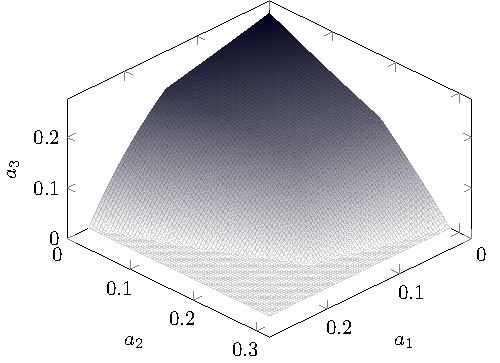
\includegraphics[width=\textwidth]{Figures/Ch7_theorem_stab.pdf}
    \else
        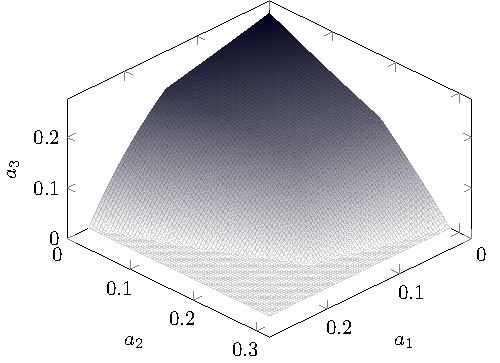
\includegraphics[draft,width=\textwidth]{Figures/Ch7_theorem_stab.pdf}
    \fi
    \caption{Stability region $\cal{R}$ according to Theorem~\ref{TH:STABILITY} for $p_1 = 1/3$, $p_2 = 2/3$, $p_3 = 1$, $\psi_1\lambda_1=1$, $\psi_2\lambda_2=2$, $\psi_3\lambda_3=3$, $\psi_1/P_1 = 1/3$, $\psi_2/P_2 = 1/2$, $\psi_3/P_3= 1$.}
\label{fig:ThStab}
\end{subfigure}%
\begin{subfigure}{.05\textwidth}
\hspace{.05\textwidth}
\end{subfigure}%
\begin{subfigure}[t]{.45\textwidth}
  \centering
    \if\printfig1
        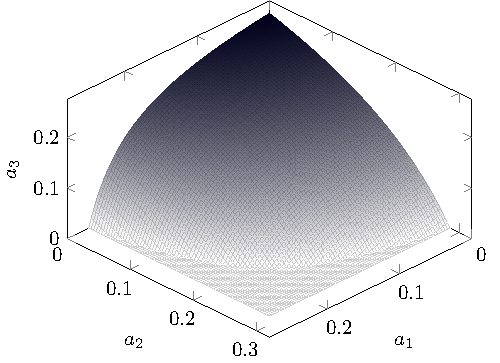
\includegraphics[width=\textwidth]{Figures/Ch7_corollary_stab.pdf}
    \else
        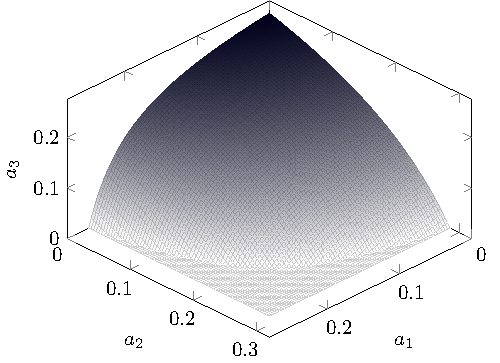
\includegraphics[draft,width=\textwidth]{Figures/Ch7_corollary_stab.pdf}
    \fi
    \caption{Maximum stability region $\cal{S}_0$ according to Corollary~\ref{cor:stab} for $p_1 = 1/3$, $p_2 = 2/3$, $p_3 = 1$,  $\psi_1\lambda_1=1$, $\psi_2\lambda_2=2$, $\psi_3\lambda_3=3$.}
\label{fig:CorStab}
\end{subfigure}
\caption{}
\end{figure}

From now on, we assume that whenever there is a packet in the buffer, the corresponding transmitter attempts to transmit, i.e., the medium access probability $p_n=1$ for all $n\in\cal{C}$.
%
We discuss in Section~\ref{sec:high-mobility} the validity of this assumption and the high-mobility assumption. The motivation is that, when the access probability of all classes is equal to one, we maximize the stability region $\cal{R}$.
%
This is easy to see with the inequalities of Theorem~\ref{TH:STABILITY}, where the right-hand side does not depend on $p_n$ and the left-hand side decreases monotonically with $p_n$. Thus, the stability region is maximized when $p_n=1$ for all $n\in\cal{C}$. The same occurs in Corollary~\ref{cor:stab}.
%
This result is surprising and might be explained by the fact that we have independence between adjacent time slots and, therefore, for each time slot there is a new scenario (a new effective PPP).
%
Then, it makes sense to always try retransmission. This approach also minimizes the mean delay according to \eqref{eq:Dn}, since the success probability $p_{s,n}$ in \eqref{eq:psn} does not depend on the access probability in a stable network.

Using Proposition \ref{prop:psk}, Proposition~\ref{prop:identity_1} is introduced, which presents an equation that relates all performance parameters independently of the transmission powers. Also, the conditions for stability are extensively simplified, see Corollary~\ref{cor:stab}.
%
\begin{proposition} \label{prop:identity_1}
	If the network is stable and $p_n=1$ for all ${n\in\cal{C}}$, then the following identities hold (at stationary state):
    \begin{equation}\label{eq:identity_1}
    	\sum_{n\in\cal{C}} \psi_n\,\lambda_n\,\dfrac{D_n}{D_n-1}\,\dfrac{a_n}{1-a_n} = 1,
    \end{equation}
    and
    \begin{equation*}
    	\frac{\psi_j}{P_j^\delta}
        \left( \frac{D_j}{D_j-1}\,\frac{1}{1-a_j} - 1\right) =
        \frac{\psi_k}{P_k^\delta} \left( \frac{D_k}{D_k-1}\,
        \frac{1}{1-a_k} - 1 \right)
        \quad \forall\,j,k\in\cal{C}.
    \end{equation*}
\end{proposition}

\begin{proof}
	We start with the terms of the sum,
	\begin{align*}
		\psi_n\,\lambda_n\,\dfrac{D_n}{D_n-1}\,\dfrac{a_n}{1-a_n}
        &\stackrel{\text{(i)}}{=} \psi_n\lambda_n\dfrac{a_n}{1-p_{s,n}}\\ 
		&= P_n^\delta \dfrac{\lambda_n\,a_n}{p_{s,n}} \left( 
        \dfrac{\psi_n}{P_n^\delta} \dfrac{p_{s,n}}{1-p_{s,n}} \right)\\
        &\stackrel{\text{(ii)}}{=} \frac{ P_n^\delta\frac{\lambda_n\,a_n}{p_{s,n}} }
        { \sum_j P_j^\delta\frac{\lambda_j\,a_j}{p_{s,j}} },
	\end{align*}
    where (i) comes from \eqref{eq:Dn} with $p_n=1$ and (ii) comes from \eqref{eq:psk_equivalence}. Summing over $\cal{C}$ ends the proof of the first identity.
    %
    For the second relation of Proposition~\ref{prop:identity_1}, we use \eqref{eq:Dn} once again to find
    \begin{equation*}
    	\dfrac{\psi_n}{P_n^\delta} \left( \dfrac{D_n}{D_n-1}\,\dfrac{1}{1-a_n} - 1\right) = \dfrac{\psi_n}{P_n^\delta} \dfrac{p_{s,n}}{1-p_{s,n}}.
    \end{equation*}
    Comparing this expression with \eqref{eq:Pi_Pk} ends the proof.
\end{proof}

Proposition~\ref{prop:identity_1} is an elegant form to see that a channel is a limited resource regarding traffic intensity and delay. Let us rewrite the identity \eqref{eq:identity_1} in terms of physical parameters,
\begin{equation} \label{eq:physical}
	\sum_{n=1}^N 4\,\lambda_n\,\overline{R}_n^2\,\theta_n^{2/\alpha}\,\dfrac{D_n}{D_n-1}\,\dfrac{a_n}{1-a_n} = \dfrac{\sin(2\pi/\alpha)}{2\pi/\alpha}.
\end{equation}
%
Note that $\frac{a_n}{1-a_n}$ and $\frac{\sin(2\pi/\alpha)}{2\pi/\alpha}$ are monotonic increasing functions and $\frac{D_n}{D_n-1}$ is a monotonic decreasing function. The right hand-side of \eqref{eq:physical} can be seen as the amount of resource available to all users of the channel.
%
Larger $\alpha$ results in higher   $\frac{\sin(2\pi/\alpha)}{2\pi/\alpha}$, meaning that a larger amount of resource is available to users. This can be explained by recalling that a larger path loss exponent leads to stronger isolation among links sharing the channel and, consequently, more users can be accommodated in the network.
%
Therefore, the larger the path loss exponent $\alpha$, the larger (smaller) the terms $\lambda_n$, $\overline{R}_n$, $\theta_n$, $a_n$ ($D_n$) can be. The identity \eqref{eq:physical} also tells us that the $n$th class of user takes a well-defined portion of the amount of resource available in the network, which is given by the $n$th term in the summation. 
%
This means that the values of $\lambda_n$, $\overline{R}_n$, $\theta_n$, $a_n$ and $D_n$ for a given class $n$ can be adjusted, while keeping the quantity $\lambda_n\,\overline{R}_n^2\,\theta_n^{2/\alpha}\,\frac{D_n}{D_n-1}\,\frac{a_n}{1-a_n}$ unchanged.
%
For instance, we can make a direct exchange between decreasing the delay $D_n$ and decreasing the arrival rate of packets $a_n$ (by controlling the ratio of transmit power levels), such that the term $\frac{D_n}{D_n-1}\,\frac{a_n}{1-a_n}$ remains constant; or else, increase the arrival rate of packets and decrease the density of users, such that the term $\lambda_n\,\frac{a_n}{1-a_n}$ remains constant. 
%
Therefore, Proposition \ref{prop:identity_1} reveals, through a simple expression, the interplay among traffic intensity, mean delay, density of users, link distance, and outage probability, when the network is stable.

\begin{remark}
    Corollary~\ref{cor:stab} and Proposition~\ref{prop:identity_1} are the simplest and the most meaningful results of the present chapter, as they translate the behavior of the network in simple equations, which do not directly depend on the transmission powers.
\end{remark}


\begin{figure}
\centering
\begin{subfigure}[t]{.45\textwidth}
  \centering
    \if\printfig1
        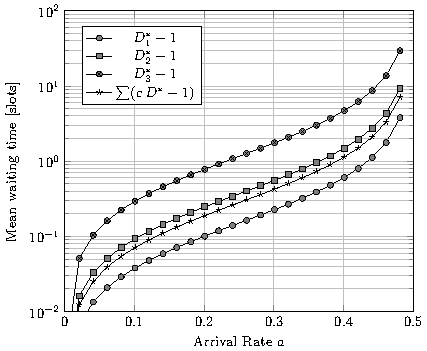
\includegraphics[width=\textwidth]{Figures/Ch7_Opt_Delay_equal_a.pdf}
    \else
        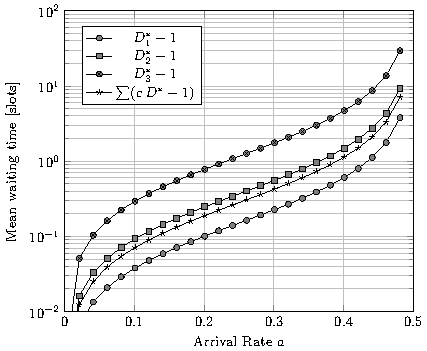
\includegraphics[draft,width=\textwidth]{Figures/Ch7_Opt_Delay_equal_a.pdf}
    \fi
    \caption{Optimum delays}
\label{fig:Opt_Delay_equal}
\end{subfigure}%
\begin{subfigure}{.05\textwidth}
\hspace{.05\textwidth}
\end{subfigure}%
\begin{subfigure}[t]{.45\textwidth}
  \centering
    \if\printfig1
        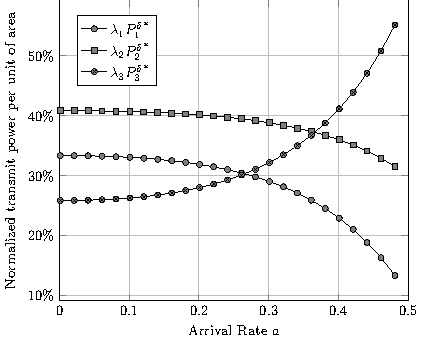
\includegraphics[width=\textwidth]{Figures/Ch7_Opt_Power_equal_a.pdf}
    \else
        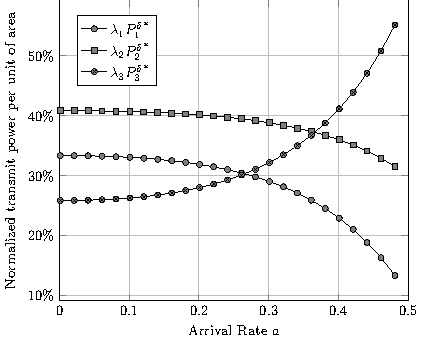
\includegraphics[draft,width=\textwidth]{Figures/Ch7_Opt_Power_equal_a.pdf}
    \fi
    \caption{Optimum transmit powers}
\label{fig:Opt_Power_equal}
\end{subfigure}
\caption{These figures represent the optimization of a 3-class network with the following parameters: $a_1=a_2=a_3=a$, $\psi_1\,\lambda_1 = 0.1$, $\psi_2\,\lambda_2 = 0.3$, $\psi_3\,\lambda_3 = 0.6$ and $c_1 = \frac{10}{16},~ c_2 = \frac{5}{16},~ c_3 = \frac{1}{16}$.}
\label{fig:opt}
\end{figure}

% % % % % % % % % % % % % % % % % % % % % % % % % % % % % %
\subsection{Interpretation and Application}
\label{sec:application}

In this section, we solve two optimization problems using the proposed formulation applied to scenarios of different classes of terminals sharing a radio channel.

% -------------------------------- %
\subsubsection{Delay Optimization}
\label{ssec:opt_delay}

Let us consider the scenario with $N$ classes sharing a channel. Each class may represent a particular user application, with each application having a different delay requirement in the network.
%
Let us suppose we are interested in adjusting the transmit power of each user class, such that the weighted average delay among all classes is minimized.
%
This problem is addressed as follows. For fixed arrival rates of vector $\bm{a}$ that satisfies Corollary~\ref{cor:stab}, i.e., for $\bm{a}\in\cal{S}_0$, let us minimize the delays $\bm{D}$ by changing the ratio between the transmit powers $\bm{P}$.
%
Each user class requires a different response time, then we weight the optimization problem with the vector $(c_1,c_2,\dots,c_N) \in \R_+^N$. The larger the coefficient of a class, the smaller the resulting mean delay to deliver packets for that class. Then, we have
\begin{equation} \label{eq:opt_prob}
	\min_{\bm{P}\in\R_+^N} \sum_{n\in\cal{C}} c_n D_n
    = \min_{\bm{P}\in\R_+^N} \sum_{n\in\cal{C}} \frac{c_n\,(1-a_n)}
        	{\left( 1 + \frac{\psi_n}{P_n^\delta}
        	\frac{\sum_j P_j^\delta\,a_j\lambda_j}
        	{1 - \sum_j \psi_j\,a_j\lambda_j} \right)^{\hspace{-1mm}-1}\!\!\! - a_n},
\end{equation}
where $D_n$ is given by Proposition~\ref{prop:psk}. Note that as thermal noise is not considered in our model, we have a degree of freedom for the optimum solution $\bm{P}^*$, which agrees with the formulation in \eqref{eq:opt_prob}.

\begin{proposition} \label{prop:opt}
	The minimum of the optimization problem \eqref{eq:opt_prob} is attained by
    \begin{equation} \label{eq:opt_D}
        {P_n^*}^\delta
        	= \dfrac{\beta}{\lambda_n a_n} \left( \frac{a_n\,\cal{A}_n}
            {1 - \sum_{k} \cal{A}_k }
            + \frac{\sqrt{c_n\,\cal{A}_n}}
            { \sum_{k} \sqrt{c_k\,\cal{A}_k } } \right), \quad n\in\cal{C},
    \end{equation}
    where $\beta$ is any positive real constant, $\cal{A}_n \triangleq \psi_n\,\lambda_n\,\frac{a_n}{1-a_n}$ and the sums are over $\cal{C}$.
\end{proposition}

\begin{proof}
	Since we have one degree of freedom for the solution $\bm{P}^*$, let us set $\sum_j P_j^\delta\,a_j\lambda_j = 1 - \sum_j \psi_j\,a_j\lambda_j$ to extensively simplify the algebraic manipulations. Then, we use the Karush-Kuhn-Tucker conditions \cite[Section~3.3.1]{bertsekas1999nonlinear} in the \emph{Lagrangian} function
    \begin{equation*}
    \begin{split}
    	\cal{L}(\bm{P},\mu) 
    	    &= \sum_{n\in\cal{C}} \frac{c_n (1-a_n)}
        	    {\left( 1 + \frac{\psi_n}{P_n^\delta}\right)^{-1}\! - a_n} + \mu\left[ \sum_{j\in\cal{C}} P_j^\delta\,a_j\lambda_j 
            	- \left(1 - \sum_{j\in\cal{C}} \psi_j\,a_j\lambda_j\right) \right],
    \end{split}
    \end{equation*}
    where $\mu\in\R$ is the \emph{Lagrange} multiplier.
    %
    The objective function is strictly convex (the Hessian is a diagonal matrix with positive eigenvalues) and the feasible region is a hyperplane, therefore the solution is the global optimum.
    %
    Now, we return to the original problem that does not have the artificial constraint. Thus, we multiply the solution by an arbitrary constant $\beta>0$ to obtain the general solution.
\end{proof}

It is interesting to note that ${\sum_k\cal{A}_k<1}$ by Corollary~\ref{cor:stab}. Therefore, ${P_n^*}^\delta$ is always a positive quantity.
%
Also, if $c_n = \cal{A}_n$ for all $n\in\cal{C}$, then the optimum delays are all equal and given by ${D_1 = D_2 = \cdots = D_N = \left( 1 - \sum_k \cal{A}_k \right)^{-1}}$. Thus, we can always choose transmit powers, such that we have the same mean delay for all classes!


As an example, let us consider a 3-class network, where Class 1 has a more restrictive delay requirement than Class 2, which is more restrictive than Class 3. We consider that all classes have the same arrival rate of packets, i.e., $a_1=a_2=a_3=a$. Figure~\ref{fig:Opt_Delay_equal} shows the expected waiting time of a packet before a successful transmission, which is $D_n^*-1$, ($n = 1,2,3$) since a transmission takes exactly one time slot. As expected, the optimization resulted in monotonic increasing functions and $D_1^* < D_2^* < D_3^*$ for all $a$.


Figure~\ref{fig:Opt_Power_equal} shows the normalized\footnote{Whenever we refer to normalized $b_n {P_n^*}^\delta$, it means that we choose $\beta$ in Proposition~\ref{prop:opt} such that $\sum_k b_k {P_k^*}^\delta = 1$ and $b_n$ is any term that depends on $n$, for example $b_n = \lambda_n$ or $b_n = a_n \lambda_n$.} transmit powers per unit of area $\lambda_n {P_n^*}^\delta$ as a function of $a$. In this case, we do not have a clear hierarchy among the transmit powers, as it depends on the traffic intensity. For $n\in\cal{C}$, if the network is close to saturation, i.e., $\sum_k\cal{A}_k$ tends to 1, then the normalized $\lambda_n {P_n^*}^\delta$ approaches $\cal{A}_n/\sum_k\cal{A}_k$ and, at first order, it does not depend on the coefficients $c_1, c_2, \dots, c_N$. On the other hand, if the network is at low traffic, i.e., $\sum_k\cal{A}_k$ tends to 0, then the normalized $a_n \lambda_n {P_n^*}^\delta$ approaches $\sqrt{c_n\cal{A}_n}/\sum_k\sqrt{c_k\cal{A}_k}$.

% -------------------------------- %
\subsubsection{Throughput Optimization}

Now, let us maximize the total throughput of the channel per unit of area with the constraint that the system is stable.
%
Since each transmitter performs retransmissions until the packet is correctly received by the intended receiver, then all packets are successfully transmitted (eventually) in a stable system. Thus, the throughput per transmitter is given by the packet arrival rate $a_n$.
%
The density of users per unit of area is given by $\lambda_n$, then the throughput of the $n$th user class per unit of area is simply $\mathscr{T}_n = \lambda_n\,a_n$ and the throughput per unit of area of the entire system $\mathscr{T}$ is the sum of the throughput for all classes $n\in\cal{C}$.

Using Corollary~\ref{cor:stab}, we can formulate the optimization problem as
${\displaystyle\max_{\bm{a}\in\cal{S}_0}} \sum_{n} \lambda_n\,a_n$.
%
However, the strict inequality in the region $\cal{S}_0$ of Corollary~\ref{cor:stab} results in an optimization problem that is not well-posed. In this case, if the optimum solution lies in the boundary of the feasible region, then the solution does not exist.
%
To circumvent this problem, we propose a new region $\cal{S}_\epsilon\subset\cal{S}_0$ by adding an arbitrarily small parameter $\epsilon \in (0,1)$ in the inequality, i.e., the new region is given by
\begin{equation*}
	\cal{S}_{\epsilon} = \left\lbrace \bm{a}\in[0,1)^N \bigm\vert \sum_{n\in\cal{C}} \psi_n\,\lambda_n\,\dfrac{a_n}{1-a_n} \le 1-\epsilon \right\rbrace.
\end{equation*}
%
As the parameter $\epsilon$ increases, the system becomes less sensitive to perturbations\footnote{When the system parameters suffer a sufficiently small change, the system remains stable.}.
Now, the optimization problem is posed as
\begin{equation} \label{eq:opt_thr}
	\max_{\bm{a}\in\cal{S}_\epsilon} \mathscr{T} = \max_{\bm{a}\in\cal{S}_\epsilon} \sum_{n\in\cal{C}} \lambda_n\,a_n.
\end{equation}
%
The following proposition presents the solution to the optimization, i.e., the optimum arrival rates $\bm{a}^*$ that maximize the throughput per unit of area and maintain the system stable.

\begin{proposition} \label{prop:eps}
	If 
    \begin{equation} \label{eq:opt_req}
		\sum_{k\in\cal{C}}\lambda_k\psi_k\left(\sqrt{\frac{\max_n \psi_n}{\psi_k}}-1\right)<1-\epsilon,
	\end{equation} then the solution of \eqref{eq:opt_thr} is attained by
    \begin{equation}
    	a_n^* = 1 - \frac{\sum_k \lambda_k \sqrt{\psi_n\psi_k}}{1-\epsilon+\sum_k\lambda_k\psi_k}, \quad n\in\cal{C},
    \end{equation}
    where the sums are over $\cal{C}$. If the inequality \eqref{eq:opt_req} is not satisfied, then the $m$th class is excluded, where $m = \arg\max_n \psi_n$, and the inequality is checked again.
\end{proposition}

\begin{proof}
	It is a direct application of the Karush-Kuhn-Tucker conditions \cite[Section~3.3.1]{bertsekas1999nonlinear} in the \emph{Lagrangian} function
    \begin{align*}
    	\cal{L}(\bm{a},\mu) = \sum_{n\in\cal{C}} \lambda_n a_n + \mu \left[ \sum_{k\in\cal{C}}\psi_k\lambda_k\frac{a_k}{1-a_k} - (1-\epsilon)\right],
    \end{align*}
    where $\mu\in\R$ is the Lagrange multiplier associated with the constraint of stability. Equation~\eqref{eq:opt_req} guarantees that the solution $\bm{a}^*\in[0,1)^N$.
    %
    The objective function is convex (affine function) and the region $\cal{S}_\epsilon$ is strictly convex because the Hessian of the function that defines the region is a diagonal matrix with negative eigenvalues. Therefore the presented solution is the global optimum and it is unique.
\end{proof}

In the optimization \eqref{eq:opt_thr}, we still have freedom to choose the transmit powers $\bm{P}$, as long the network remains stable. The best way of choosing $\bm{P}$ is by minimizing the delays, which we have already done in Subsection~\ref{ssec:opt_delay}, Proposition~\ref{prop:opt}, where the arrival rates $\bm{a} \in \cal{S}_\epsilon \subset \cal{S}_0$ are fixed. When the optimization is performed in this sequence (maximization of throughput, then minimization of delay), we have the optimum throughput (per unit of area) and the optimum delays for the optimum configuration of arrival rates.
%%
Later in this section, we illustrate this procedure with a numerical example.

In order to solve the optimization problem \eqref{eq:opt_thr} we did not have to handle with the transmit powers $\bm{P}$ directly, which would make the solution and the problem formulation more cumbersome. This shows the usefulness of Corollary~\ref{cor:stab}.

\begin{figure}
\centering
\begin{subfigure}[t]{.45\textwidth}
  \centering
    \if\printfig1
        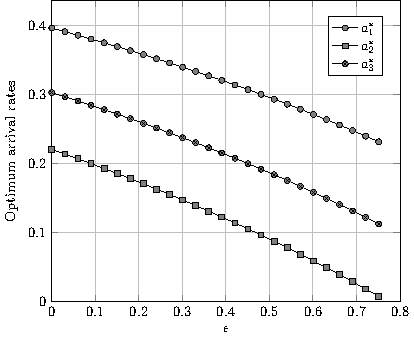
\includegraphics[width=\textwidth]{Figures/Ch7_Opt_a_eps.pdf}
    \else
        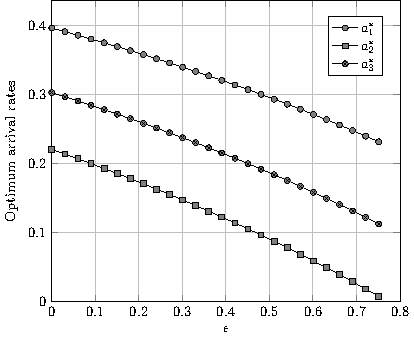
\includegraphics[draft,width=\textwidth]{Figures/Ch7_Opt_a_eps.pdf}
    \fi
    \caption{Optimum arrival rates}%
    \label{fig:Opt_a_eps}
\end{subfigure}%
\begin{subfigure}{.05\textwidth}
    \hspace{.05\textwidth}
\end{subfigure}%
\begin{subfigure}[t]{.45\textwidth}%%
  \centering
    \if\printfig1
        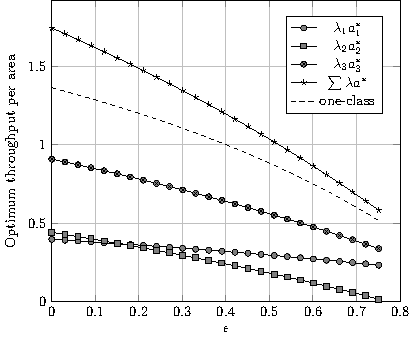
\includegraphics[width=\textwidth]{Figures/Ch7_Opt_lam_a_eps.pdf}
    \else
        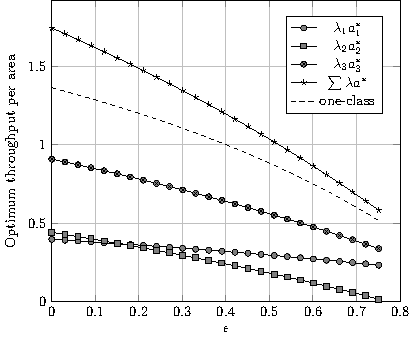
\includegraphics[draft,width=\textwidth]{Figures/Ch7_Opt_lam_a_eps.pdf}
    \fi
    \caption{Optimum throughput. The dashed curve corresponds to a scenario with only the best performing class}
    \label{fig:Opt_lam_a_eps}
\end{subfigure}
%
\begin{subfigure}[t]{.45\textwidth}%%%
  \centering
    \if\printfig1
        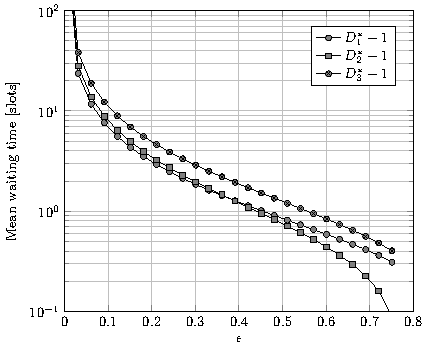
\includegraphics[width=\textwidth]{Figures/Ch7_Opt_D_eps.pdf}
    \else
        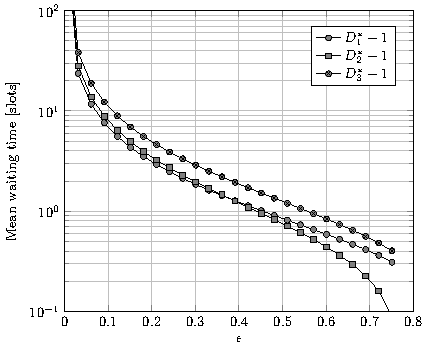
\includegraphics[draft,width=\textwidth]{Figures/Ch7_Opt_D_eps.pdf}
    \fi
    \caption{Optimum delays}
    \label{fig:Opt_D_eps}
\end{subfigure}%
\begin{subfigure}{.05\textwidth}
    \hspace{.05\textwidth}
\end{subfigure}%
\begin{subfigure}[t]{.45\textwidth}%%%%
  \centering
    \if\printfig1
        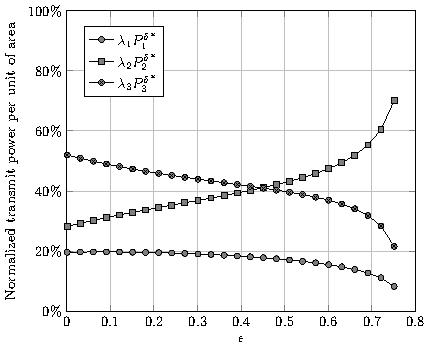
\includegraphics[width=\textwidth]{Figures/Ch7_Opt_P_eps.pdf}
    \else
        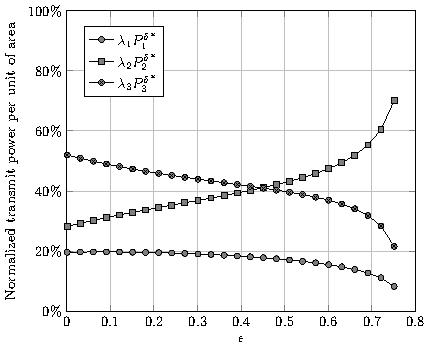
\includegraphics[draft,width=\textwidth]{Figures/Ch7_Opt_P_eps.pdf}
    \fi
    \caption{Optimum transmit powers}
    \label{fig:Opt_P_eps}
\end{subfigure}
\caption{These figures represent the optimization of the throughput and mean delay of a 3-class network with the parameters given in Table~\ref{tab:param}.}
\label{fig:opt_eps}
\end{figure}

Let us illustrate the throughput optimization problem with a system for which the parameters are shown in Table~\ref{tab:param}. Figure~\ref{fig:Opt_a_eps} shows the optimum arrival rates $\bm{a^*}$ that maximizes the throughput per unit of area.
%
\begin{table}[hbt]
  \centering
  \caption{Network parameters for Fig.~\ref{fig:opt_eps}}
  \begin{tabular}{l l}
        \hline
      \hline
      \textbf{Parameters} & \textbf{Values} \\
      \hline
        $(\lambda_1,\lambda_2,\lambda_3)$	& $=(1,2,3)$ \\
        $(\psi_1,\psi_2,\psi_3)$			& $=(0.3,0.5,0.4)$ \\
		$(c_1,c_2,c_3)$						& $=(\frac{1}{3},\frac{1}{3},\frac{1}{3})$ \\
      \hline
      \hline
  \end{tabular}
  \label{tab:param}
%   \vspace*{-\baselineskip}
\end{table}
%
It is quite interesting that the optimum solution is not (necessarily) exclusively activating the class with the best link quality (i.e., the class with the smallest $\psi$, which is Class 1 in this example). In Fig.~\ref{fig:Opt_lam_a_eps} it is shown the optimum throughput for each class and the total throughput of the system.
%
For comparison, we plotted a dashed curve representing the total throughput if we only use the best performing user class, regarding throughput.
The dashed curve is below the optimum total throughput for all $\epsilon$. Therefore, the best solution is always a combination of all user classes, as long as \eqref{eq:opt_req} is satisfied.
%
On the other hand, if this equation is not satisfied, it means that there is at least one user class with a bad link quality, such that it is better (regarding throughput efficiency) to reallocate this user class to another channel.

Now that we have, for each $\epsilon$, the arrival rate configuration $\bm{a}^*(\epsilon)$ which gives the maximum throughput, we can use Proposition~\ref{prop:opt} to find the best configuration of transmit powers $\bm{P}^*(\epsilon)$ that minimizes the sum of the mean delays for each optimum configuration of arrival rates $\bm{a}^*(\epsilon)$.
%
Figure~\ref{fig:Opt_D_eps} shows the result of this optimization, which is a direct application of \eqref{eq:opt_D}.
%
It is worth noting that as we increase $\epsilon$ the system is farther from instability, which corresponds to having a smaller delay to transmit packets, as we can see in Fig.~\ref{fig:Opt_D_eps}, and a smaller throughput, as shown in Fig.~\ref{fig:Opt_lam_a_eps}.
%
Figure~\ref{fig:Opt_P_eps} shows the optimum distribution of power per unit of area required by each user class. Notice that the first user class, which has the best link quality, uses the smallest power per unit of area. However, this behavior is more intricate; it also depends on the density of users of the corresponding class. Notice, for example, the inversion between user classes 2 and 3 as we increase $\epsilon$ in Fig.~\ref{fig:Opt_P_eps}.

Another interesting and direct result from Corollary~\ref{cor:stab} is to provide an upper bound for the total throughput per unit of area $\mathscr{T}$ in a stable system, which is given by $1/(\min_n\psi_n)$.
%
This is not a tight bound, however it is interesting on its own, due to its simplicity and the fact that it does not depend on the density of users. The proof follows
\begin{align}
	\mathscr{T} = \sum_{k\in\cal{C}} a_k\lambda_k &\le \frac{1}{\min_{n}\psi_n} \sum_{k\in\cal{C}} \psi_k\,a_k\,\lambda_k \nonumber\\
        &< \frac{1}{\min_{n}\psi_n} \sum_{k\in\cal{C}}\psi_k\,\lambda_k\,\frac{a_k}{1-a_k} \nonumber\\
        &< \left(\textstyle\min_{n}\psi_n \right)^{-1},
\end{align}
where the last inequality comes from Corollary~\ref{cor:stab}.

% % % % % % % % % % % % % % % % % % % % % % % % % % 
% % % % % % % % % % % % % % % % % % % % % % % % % % 
\section{On the High-mobility Assumption} \label{sec:high-mobility}

In this section, we address the high-mobility assumption, which may not be realistic in real wireless networks, since the mobility of transmitters does not change drastically between adjacent time slots. Therefore, the independence assumption would not hold.
%
Nevertheless, in a stable wireless network that has a small packet arrival rate $a$ per user or a small access probability $p$, the correlation might be sufficiently small such that the independence (high-mobility) assumption is reasonable. In \cite{haenggi2013diversity} the authors show that if the access probability $p$ is sufficiently small, then the independence assumption provides a good approximation.

When the packet arrival rate $a$ or the access probability $p$ are small, the typical user sees a significantly different PPP of transmitters for each time slot, which justifies the independence (high-mobility) assumption. We verified this claim through simulations and the result is shown in Fig.~\ref{fig:high-mobility}, where it is used one user class with ${\lambda c \overline{R}^2 = \pi/4}$, ${\alpha = 3}$ and ${\theta = 1}$.
%
\begin{figure}
    \centering
    \if\printfig1
        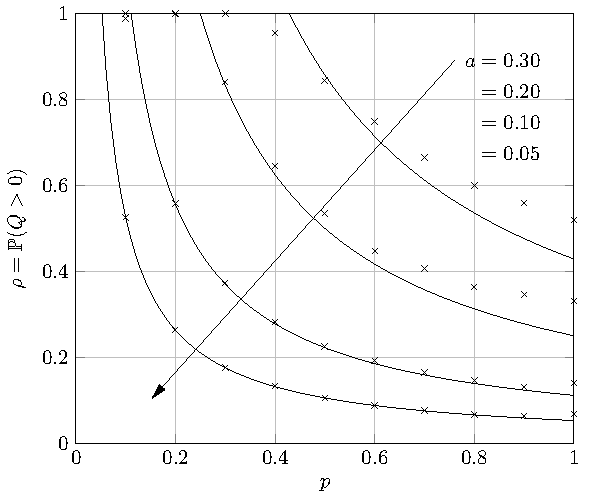
\includegraphics[width=0.55\textwidth]{Figures/Ch7_high-mobility.pdf}
    \else
        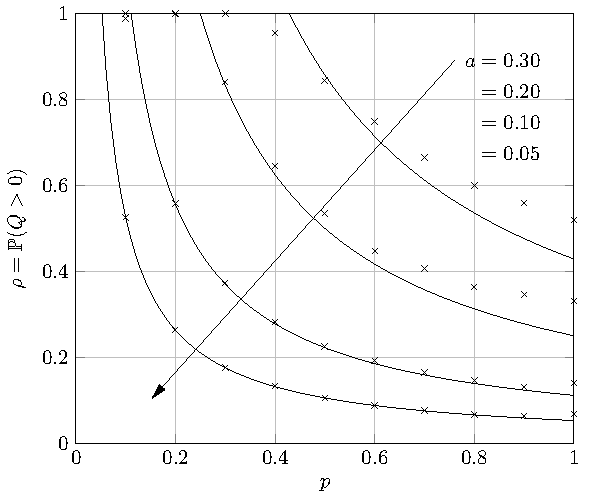
\includegraphics[draft,width=0.75\textwidth]{Figures/Ch7_high-mobility.pdf}
    \fi
    \caption{Queue load $\rho$ as a function of the access probability $p$. Simulation results with a static network are presented in marks and the theoretical results with the high-mobility assumption are presented in curves.}
    \label{fig:high-mobility}
\end{figure}

The mean load of the queues $\rho$, which is equivalent to the percentage of queues with packets to transmit, are plotted as a function of the access probability $p$ for several values of arrival rate $a$. As expected, for small values of $a$ or $p$, the theoretical model presents good estimations of the average queue load.
%
It is important to emphasize that we did not plot the mean delay $D$, because in a static PPP there might exist a set of unstable users, whose queues and delays tend to infinity. This would raise the average delay to infinity too. Then, we chose to plot the mean load $\rho$, which is equal to 1 for unstable users and does not tend to infinity opposed to the mean delay $D$.

To establish Proposition~\ref{prop:identity_1}, we supposed that the access probability $p$ is equal to one for all users. In the context of high-mobility, this approach makes sense, since the typical user sees a different interference scenario for each time slot. Thus, it is reasonable to attempt a retransmission every time slot until the packet is successfully transmitted. This also minimizes the mean delay $D$, which is in accordance with \eqref{eq:Dn}, as the transmission success probability $p_{s,n}$ does not depend on the access probability $p_n$ in a stable network.

There is another scenario, which does not require high-mobility to achieve spatial independence between adjacent time slots. This scenario is a network that uses the frequency-hopping scheme over a set of channels \cite{tse2005fundamentals}. For each time slot, there is a different PPP pattern, since the transmitting nodes select with equal probability one channel to transmit. Thus, the spatial correlation between time slots decreases with the number of channels available for selection.

% % % % % % % % % % % % % % % % % % % % % % % % % % 
% % % % % % % % % % % % % % % % % % % % % % % % % % 
\section{Bandwidth Partitioning on High-mobility Bipolar Networks}
\label{sec:bandwidth}

In this section, we consider the model presented in Section~\ref{sec:N-class} with only two classes of users, i.e., $N=2$.
%
However, differently from our previous models, the available frequency band is partitioned among users of one of the classes, such that users of this class can access only a fraction of the original bandwidth available to the network at a time.
%
The other class continues using the whole frequency band available.
%
The motivation for such bandwidth partitioning is to reduce the interference among users, leading to a higher network capacity.

The work presented in this section generalizes the paper by Jindal et al. in \cite{jindal2008bandwidth} in the sense that it (\textit{i}) considers two user classes and (\textit{ii}) investigates the effects of bandwidth partitioning on the mean \textit{queuing} delay.
%
By considering two classes of users, we are able to study the performance of a network in which users of one class are allowed to transmit on a fraction of the channel accessed by users of the other class. Also, by studying the delay, we are able to have a better understanding of the effects of bandwidth partitioning on network performance.
%
% The present work also extends the study presented in \cite{dester2018} by using bandwidth partitioning on one of the user classes. 
% More specifically, we recover some results from \cite{jindal2008bandwidth} and \cite{dester2018} by setting the arrival rate of Class 2 $a_2 = 0$ and by setting the number of band partitions $M=1$, respectively.

We used the wireless network formulation proposed in Section~\ref{sec:N-class} to achieve a tractable framework for the analysis of the bandwidth partitioning.

The main contributions presented in this section can be summarized as follows:
\begin{itemize}
    \item We have found a pair of simple equations that relate the main parameters of the network and guarantees network stability (Theorem~\ref{th:identity});
    \item A transcendental equation to find the optimum Class 1 spectral efficiency is derived, along with the optimum number of partitions (Theorem~\ref{th:optimum_eta});
    \item The first-order expansion of the optimum spectral efficiency around a small use of the channel by Class 2 (Eq.~\eqref{eq:eta_expansion});
    \item We show that the bandwidth partitioning strategy is more effective when the path loss exponent is not small and the performance requirements of Class 2, the one whose users access the whole bandwidth, is not high in respect to the maximum performance attainable (Fig.~\ref{fig:a_ratio}).
\end{itemize}

% The paper is organized as follows. In Section~\ref{sec:sysmod_M} the system model is presented and in Section~\ref{sec:stab} we derive the stability conditions and expressions for stationary transmission success probability and mean delay. Using these expressions, we present in Section~\ref{sec:opt} the optimization problem involving bandwidth partitioning and proves the existence and uniqueness of the solution.  Section~\ref{sec:num} provides some numerical examples of bandwidth optimization. %, also including a case involving cellular and D2D.
% Section~\ref{sec:conc} concludes the paper.

% % % % % % % % % % % % % % % % % % % % % % % % % % % % % %
\subsection{System Model} \label{sec:sysmod_M}

We consider the network model presented in Section~\ref{sec:N-class} with two user classes (namely Class 1 and Class 2), and only one and important difference that users of Class 1 access a fraction of the bandwidth during each transmission.

%The high-mobility model, which is used in several works (see, for instance \cite{jindal2008bandwidth}, \cite{baccelli2010stochastic}, \cite{stamatiou2010random}, \cite{dester2018}), assumes that users occupy a different point in space for each time slot. 
%The communication protocol is the slotted Aloha, i.e., for each time slot, if a source (transmitter) has packets to transmit, it will transmit one packet with a fixed probability, independently from other sources and the past. The position of source $i \in \N$ of class $n\in\{1,2\}$ at time $t\in\N$ is denoted by $X_{i,n}(t) \in \R^2$. We assume that $\{X_{i,n}(t)\}_i\subset \R^2$ is a marked homogeneous Poisson point process (PPP) of density $\lambda_n$. These PPPs are independent across classes and time slots. The transmit power of a source of class $n$ is denoted by $P_n$, assumed to be constant over time slots and the same for all sources within a class.
%
% Let $Y_{i,n}(t)\in\R^2$ be the position of the destination terminal with which the $i$th source of class $n$ communicates. The distribution of $Y_{i,n}(t)$ is such that the location of the destination terminal is at a random distance $R_{i,n}(t) = ||X_{i,n}(t) - Y_{i,n}(t)||$ from the corresponding transmitter in a uniformly random direction, where $||\cdot||$ is the euclidean norm. We assume that $R_{i,n}(t)$ is iid across time slots and users, and it follows a Rayleigh distribution of mean $\overline{R_n}$.
%
% This assumption contributes to the tractability of the model and it was also used in \cite{dester2018, lin2014spectrum, di2014stochastic}. In this context, a reasonable assumption is to consider an interference-limited network, i.e., the noise is negligible.
% It should be noted that the destination terminals are not part of the Poisson Point Processes that model the positions of the sources.

% Each source has a buffer of infinite capacity for arriving packets. The total number of packets in the $i$th source of class $n$ at time $t$ is denoted by the queue length $Q_{i,n}(t)$. If the queue of a given source is not empty, then the source tries to transmit a packet with probability $p_n$ (medium access probability) following the first-come-first-serve
% (FCFS) discipline and the transmission takes exactly one time slot.
% %
% Thus, each queue length $Q_{i,n}(t)$ forms a Markov chain (for more details, see \cite{dester2018}).
% %
% The packet is successfully transmitted when the signal-to-interference ratio (SIR) of the received signal is greater than a threshold $\theta_n$ (capture effect). In this case, the receiver sends an acknowledge through an error-free channel and the packet leaves the queue. Packets arrive at the queue according to an iid Bernoulli distribution of parameter $a_n$.
% %
% Chronologically, within each time slot, we have the transmission of packets, then the arrival of packets, and, at the end of the time slot, the displacement of the sources occurs to form a new and independent PPP realization.

% The SIR experienced by the typical user from class $n$ is given by $\mathrm{SIR}_{i,n}= P_n h_{i,n} R_{i,n}^{-\alpha}/I$, where $\alpha>2$ is the path-loss exponent, the Rayleigh fading effect is represented by the fading coefficient $h_{i,n}$, which is an iid (with respect to time and users) exponentially distributed random variable of unit mean and remains constant during the time slot, and $I$ is the aggregate interference from other sources. It is known that $\mathrm{SIR}_{i,n}$ is an iid random variable with respect to time \cite{baccelli2010stochastic}.

More specifically, the frequency band of bandwidth $B_0$ is shared by users of both classes. For Class 1 transmissions, this frequency band is divided into $M$ partitions (sub-bands) of bandwidth $B_0/M$, and each Class 1 user transmits over one randomly selected sub-band. Therefore, the density of sources for each partition becomes $\lambda_1/M$. On the other hand, users of Class 2 transmit over the whole available bandwidth $B_0$.
%
Note that front-end receiver filters of the first class destinations will capture $1/M$ of the power from transmissions of users of the second class and do not capture anything from other partitions of the first class. On the other hand, the second class destinations capture all the power coming from sources of both classes.

The transmission rate $R_T$ for the first-class users is fixed and, as in \cite{jindal2008bandwidth}, the SIR threshold\footnote{The transmission successfully happens if and only if the SIR is greater than the threshold.} $\theta_1$ comes from the following equation: ${R_T = (B_0/M)\,\ln(1+\theta_1)}$. Then, ${\theta_1 = \euler^{M\eta_0}-1}$, where ${\eta_0 \triangleq R_T/B_0}$ is the spectral efficiency without partitioning the frequency band. Note that the transmission rate for the first class of users remains unchanged with bandwidth partitioning.

% Both user classes use the same bandwidth and the goal is to find the optimum number of partitions $M$ for the first user class.
% Table~\ref{tab:symbols} summarizes the notation.

% \begin{table}[hbt]
%   \centering
%   \caption{Symbols and Definitions}
%   \begin{tabular}{ll}
%       \toprule
%       \textbf{Symbol} & \textbf{Definitions} \\
%       \midrule
%         $\alpha\in(2,\infty)$	& Path loss exponent \\
%         $\delta\in(0,1)$		& $\triangleq 2/\alpha$ \\
% 		$M \in \N$				& Number of partitions \\
%         $\eta_0 \in \R_+$		& Spectral efficiency without bandwidth partitioning \\
%         $\eta  \in \R_+$		& $\triangleq M \eta_0 $, spectral efficiency of Class 1 \\
%         $p_n\in[0,1]$   		& Medium access probability \\
%       	$a_n\in[0,1]$			& Packet arrival rate \\
%         $p_{s,n}\in[0,1]$		& Stationary transmission success probability \\
%         $\theta_n\in \R_+$		& SIR threshold for successful transmission \\
%         $D_n\in(1,\infty)$		& Average packet transmission delay \\
%         $\overline{R}_n\in \R_+$& Mean source-destination separation distance \\
%         $P_n\in \R_+$			& Transmit power \\
%         $\lambda_n\in \R_+$		& User density of class $n$\\
%         $\psi_n\in \R_+$ 		& $\triangleq 4\,\Gamma(1+\delta)\,
%          						  \Gamma(1-\delta)\,\overline{R}_n^2\,
%                                   \theta_n^{\delta}$~~(link quality)\\
% %          $||\cdot||$			& Euclidean norm \\
%         % $\ind_A(x)$				& indicator function\\
%         $\Psi_n\in \R_+$       ~& $\triangleq \psi_n\lambda_n \left(\frac{D_n}{D_n-1}\right) \left(\frac{a_n}{1-a_n}\right)$~~(resource utilization)\\
%       \bottomrule
%   \end{tabular}
%   \label{tab:symbols}
% %    \vspace*{-\baselineskip}
% \end{table}

% % % % % % % % % % % % % % % % % % % % % % % % % % % % % %
\subsection{Stability Conditions and Stationary Analysis}
\label{sec:stab}

In this section, we derive conditions for stability and carry a stationary analysis of the network, which leads to expressions relating network parameters and performance metrics. These expressions are used in Section \ref{sec:opt} to formulate an optimization problem to maximize the network performance when bandwidth partitioning is employed. 

% In order to derive the stability conditions, we first determine the successful transmission probability of a typical user from class $n\in\{1,2\}$, given the \textit{effective density of active sources} $\lambda^\mathrm{eff}_k(t)$ for each class $k\in\{1,2\}$ in a time slot $t\in\Z_+$.
% %
% The effective density of active sources of a class is the PPP density of the sources with non-empty queues and allowed by the medium access control technique to transmit a packet.
% %
% This access control is modeled in this work by the medium access probability $p_n$. One can calculate the probability of successful transmission by deconditioning the general expression for the successful probability given in \cite[Eq.~(9)]{haenggi2009stochastic} for the distance $R$, when $R$ follows a Rayleigh distribution. This was done in \cite[Proposition~1]{dester2018}. Then, the successful transmission probability is given by

From the proof of Proposition~\ref{prop:psk} in Eq.~\eqref{eq:P_SIR}, for two classes of users, we can write that%
\begin{equation} \label{eq:P_SIR_M}
	\P(\mathrm{SIR}_{i,n}(t) > \theta_n) 
    	= \nu_n\!\left( P_1^\delta\,\lambda_\mathrm{eff}^{(1)}(t)
        	+ P_2^\delta\,\lambda_\mathrm{eff}^{(2)}(t) \right), \quad t\in\N,
\end{equation}
where the function ${\nu_n: \R_+ \longrightarrow \R_+}$ is defined as
\begin{equation}\label{defNu}
\nu_n(x) \triangleq \left(1+\frac{\psi_n}{P_n^\delta}x\right)^{-1}, \quad x\in\R_+, n\in\{1,2\}.
\end{equation}

A necessary and sufficient condition for the stability of the buffers for both user classes is given by the following proposition.
%
% A system is stable whenever the Markov chain describing the system admits a proper limit distribution when $t\to\infty$ \cite{szpankowski1994stability}.
%
Stability region refers to the set of arrival rates for which the system is stable.

\begin{proposition} \label{prop:stability}
The system network is stable if and only if $(a_1,a_2) \in \mathcal{E}_1 \cup \mathcal{E}_2$, where
\begin{align*}
	\mathcal{E}_1
    	&= \left\lbrace (a_1,a_2)\in [0,1]^2 \mid
    		a_1 < p_1\,\nu_1\!\left( P_1^\delta\tfrac{\lambda_1}{M}p_1
            	+\tfrac{P_2^\delta}{M^\delta}\lambda_2 p_2\right), 
            a_2 < p_2\,\nu_2\!\left( P_1^\delta\lambda_1
        		\tfrac{a_1}{\widetilde{p}_{s,1}} + P_2^\delta\lambda_2 p_2 \right) \right\rbrace,\\
	\mathcal{E}_2
    	&= \left\lbrace (a_1,a_2)\in [0,1]^2 \mid
    		a_2 < p_2\,\nu_2\!\left( P_1^\delta\lambda_1 p_1
            	+P_2^\delta\lambda_2p_2\right), 
            a_1 < p_1\,\nu_1\!\left(P_1^\delta
        		\tfrac{\lambda_1}{M}p_1+\tfrac{P_2^\delta}{M^\delta}
                \lambda_2\tfrac{a_2}{\widetilde{p}_{s,2}} \right)
			\right\rbrace,
\end{align*}
where
\begin{equation*}
	\widetilde{p}_{s,1} = \frac{1-\psi_1\tfrac{\lambda_1}{M}a_1}
    	{1+\psi_1(\tfrac{P_2}{M P_1})^\delta\lambda_2p_2}, \qquad
    \widetilde{p}_{s,2} = \frac{1-\psi_2\lambda_2 a_2}
    	{1+\psi_2(\tfrac{P_1}{P_2})^\delta\lambda_1 p_1}.
\end{equation*}
\end{proposition}
%
\begin{proof}
	Sufficient conditions for the network stability are obtained by using the concept of dominant network \cite[Section~2.1.2]{kompella2014stable}, which corresponds to a network almost identical to the original one, differing only on the fact that users of some classes of the dominant network transmit dummy packets when their queues are empty. If the dominant network is stable, then the original network is stable as well.
	%
    Let us analyze a dominant network where both classes transmit dummy packets with the correspondent medium access probability $p_1, p_2$. In this case, the effective density of active sources for the $n$th traffic class is $\lambda_\mathrm{eff}^{(n)} = \lambda_n\,p_n$ for all $t$, since we are assuming that sources transmit dummy packets when their queues are empty.
    %
    Note that we have partitioned the frequency band of the first class of users into $M$ sub-bands, i.e., the destinations of packets of this user class only receive signals within their bandwidth, i.e., signals from $1/M$ of the sources of the first user class and $1/M$ of the power of signals the sources of the second class of users.

%    In general, a sufficient condition for stability\footnote{The system is stable if the expected rate of incoming packets is smaller than the expected number of packets leaving the queue per time slot \cite{loynes1962stability}.} for both classes are 
	A sufficient condition for stability is
    \begin{equation}
    a_n < p_n \, P(\mathrm{SIR}_{i,n} > \theta_n), \quad n\in\{1,2\},
    \end{equation}
by Loynes' theorem (Theorem~\ref{th:loynes}). Then, using Eq.~\eqref{eq:P_SIR_M}, sufficient conditions for stability for the first and the second classes are  
    \begin{equation} \label{eq:stabClass1}
    	a_1<p_1\,\nu_1\!\left[P_1^\delta\tfrac{\lambda_1}{M}p_1+\left(\tfrac{P_2}{M}\right)^\delta\lambda_2p_2\right]
    \end{equation}
    and 
    \begin{equation} \label{eq:stabClass2}
	a_2 < p_2\,\nu_2\!\left(P_1^\delta\lambda_1p_1
    	+ P_2^\delta\lambda_2p_2\right).
    \end{equation}
    If both equations \eqref{eq:stabClass1} and \eqref{eq:stabClass2} are satisfied, then the system is stable. However, the stability region described by Proposition \ref{prop:stability} can be expanded, as presented next. Let us consider two cases: (i) the arrival rate $a_1$ satisfies Eq.~\eqref{eq:stabClass1}; (ii) the arrival rate $a_2$ satisfies Eq.~\eqref{eq:stabClass2}.
\begin{enumerate}[label=(\roman*)]
    \item For this case, we consider another dominant network, where only users of the second class transmit dummy packets. We know that the first class is stable and it has a limit stationary distribution as $t\to\infty$, since we are assuming $a_1$ satisfies \eqref{eq:stabClass1}, and we want to determine a new stability condition for the second user class. We begin by noting that, in this context, the load $\rho_1$ of a queue of the first user class can be written as the ratio of the packet arrival probability and the probability a packet that leaves the queue, i.e., $\rho_1 = a_1/(p_1\widetilde{p}_{s,1})$, where $\widetilde{p}_{s,k} \triangleq \P(\mathrm{SIR}_{i,k}>\theta_k)$, $k\in\{1,2\}$, is the Class $k$ coverage probability in the dominant network. Therefore, the stationary  effective density of active sources from the first class is $\lambda_1^\mathrm{eff} = \lambda_1\,p_1\,\rho_1$. From Eq.~\eqref{eq:P_SIR_M}, we have the following fixed-point equation
    \begin{equation*}
    	\widetilde{p}_{s,1}
        	= p_1\,\nu_1\!\left[ P_1^\delta\tfrac{\lambda_1}{M}\tfrac{a_1}{\widetilde{p}_{s,1}}
            	+ \left(\tfrac{P_2}{M}\right)^\delta\!\lambda_2 p_2 \right],
    \end{equation*}
    which is easily solvable for $\widetilde{p}_{s,1}$. Then, we can use this value to derive a weaker stability condition for the second user class, i.e., $a_2<p_2\,\nu_2(P_1^\delta\lambda_1 p_1\rho_1+P_2^\delta\lambda_2 p_2)$, where $\rho_1 = a_1/(p_1\widetilde{p}_{s,1})$. This establishes the region $\cal{E}_1$.
    
    \item Analogously to case (i), we now consider a dominant network where users from the first class transmit dummy packets when their queues are empty. Following the same procedure as in the previous case, we arrive at the following fixed-point equation for the stationary successful transmission probability of the second user class,
    \begin{equation*}
    	\widetilde{p}_{s,2}
        	= p_2\,\nu_2\!\left( P_1^\delta\lambda_1 p_1
            	+ P_2^\delta\lambda_2 \tfrac{a_2}{\widetilde{p}_{s,2}} \right),
    \end{equation*}
    whose solution allows us to establish a weaker stability condition for the first class of user as
    \begin{equation}
    	a_1<p_1\,\nu_1 \left[P_1^\delta\tfrac{\lambda_1}{M}p_1+\left(\tfrac{P_2}{M}\right)^\delta\lambda_2p_2 \rho_2 \right],
    \end{equation}
    where $\rho_2 = a_2/(p_2\widetilde{p}_{s,2})$ is the load of queues from the second user class. This condition establishes region $\cal{E}_2$.
\end{enumerate}
Necessary conditions are established when we analyze the case $(a_1,a_2)\notin\cal{E}_1\cup\cal{E}_2$.
Note that, if the pair $(a_1,a_2)$ does not belong to the cases (i) or (ii), then there exists a positive probability that the original network and the dominant network, which transmits dummy packets for both classes, are \emph{indistinguishable} \cite[Section~3.2]{szpankowski1994stability} and, therefore, both systems are not stable by Loynes' Theorem (Theorem~\ref{th:loynes}). If all the queues start with a large number of packets, the original and the dominant networks behave identically with a positive probability (see \cite[Proposition~1]{stamatiou2010random}).
On the other hand, if $(a_1,a_2)$ belongs to only one of the cases (i) or (ii), then one of the classes is stable, but again with a positive probability, the original network behaves identically as the correspondent dominant network and, therefore, the other class is not stable.
\end{proof}

\begin{remark} \label{rem:stab}
The stability region in Proposition~\ref{prop:stability} is maximized when ${p_1 = p_2 = 1}$. This can be shown by noting that the two boundary inequalities that define the region $\cal{E}_1 \cup \cal{E}_2$ in the first quadrant are monotonically increasing with $p_1$ or $p_2$.
\end{remark}

Since we have established the conditions for stability, we now proceed by showing the stationary probability of successful transmission and mean delay for each user class. 

\begin{proposition}\label{prop:stationary}
	If the system is stable, then the stationary transmission success probabilities $p_{s,1}$ and $p_{s,2}$ and the stationary mean delays $D_1$ and $D_2$, for user classes 1 and 2, are given by 
\begin{gather*}
    	p_{s,1} = \frac{(1-\psi_1\tfrac{\lambda_1}{M}a_1)(1-\psi_2\lambda_2 a_2)
        	- \tfrac{1}{M^\delta}\psi_1\psi_2\lambda_1\lambda_2 a_1 a_2}
            {1+\lambda_2 a_2 \left[\psi_1\left(\tfrac{P_2}{M P_1}\right)^\delta-\psi_2\right]},\\
    	p_{s,2} = \frac{(1-\psi_1\tfrac{\lambda_1}{M}a_1)(1-\psi_2\lambda_2 a_2)
        	- \tfrac{1}{M^\delta}\psi_1\psi_2\lambda_1\lambda_2 a_1 a_2}
            {1+\lambda_1 a_1 \left[\psi_2\left(\tfrac{P_1}{P_2}\right)^\delta-\tfrac{\psi_1}{M}\right]},
     \end{gather*}  
     \begin{equation*}       
    	D_1 = \frac{1-a_1}{p_1\,p_{s,1}-a_1}, \qquad
    	D_2 = \frac{1-a_2}{p_2\,p_{s,2}-a_2}.
    \end{equation*}
\end{proposition}

\begin{proof}
	If the system is stable, then for each user class $n$, there exists the limit transmission success probability $p_{s,n}$, as $t\to \infty$. The load at a typical queue is given by $\rho_n = a_n/(p_n\,p_{s,n})$ and the effective density of active sources is $\lambda_n^\mathrm{eff}=\lambda_n p_n\rho_n$. Considering bandwidth partitioning and stationary state, we derive the following system of equations from Eq.~\eqref{eq:P_SIR_M}:
\begin{align*}
	p_{s,1} 
    	&= \nu_1\!\left[ P_1^\delta \tfrac{\lambda_1}{M} \tfrac{a_1}{p_{s,1}}
        	+\left(\tfrac{P_2}{M}\right)^\delta\!\lambda_2\tfrac{a_2}{p_{s,2}}\right],\\
	p_{s,2} 
    	&= \nu_2\!\left( P_1^\delta \lambda_1 \tfrac{a_1}{p_{s,1}}
        	+P_2^\delta \lambda_2 \tfrac{a_2}{p_{s,2}}\right),
\end{align*}
	which can be solved for $p_{s,1}$ and $p_{s,2}$. The mean delays $D_1$ and $D_2$ follow from Theorem~\ref{th:geo/geo/1} as all queues in the network can be modeled as Geo/Geo/1 queues. 
\end{proof}

Next, we provide an identity that is useful when stating the optimization problem of bandwidth partitioning in Section~\ref{sec:opt}.

\begin{theorem}\label{th:identity}
	Let $p_1=p_2=1$. The system is stable if and only if the following equations hold:
    \begin{align}
    	\frac{\Psi_1}{M} 
        	&= \frac{1-\Psi_2}{1+(M^{1-\delta}-1)\,\Psi_2}, \label{eq:theor01} \\
        \frac{P_1^\delta}{P_2^\delta}
    		&= \left(\frac{1-\Psi_2}{\Psi_1}\right) \left(\frac{\psi_1-\frac{\Psi_1}{\lambda_1 a_1}}
        		{\psi_2-\frac{\Psi_2}{\lambda_2 a_2}}\right), \label{eq:theor02} 
    \end{align}
    with $D_1, D_2 > 1$ and 
\begin{equation} \label{eq:defPsi}
\Psi_n \triangleq \psi_n\lambda_n \left(\frac{D_n}{D_n-1}\right) \left(\frac{a_n}{1-a_n}\right) \ge 0, \qquad n\in\{1,2\}.
\end{equation}    
% with $D_n\in(1,\infty)$, $n\in\{1,2\}$.
\end{theorem}

\begin{proof}
	If the system is stable, then the equations can be verified through Proposition~\ref{prop:stationary} and some manipulations. On the other hand, to prove that a set of parameters that satisfy the equations of the theorem implies stability, one can follow these steps: plug Eq.~\eqref{eq:theor02} into the inequalities of Proposition~\ref{prop:stability}; then use Eq.~\eqref{eq:theor01} and the fact that $\Psi_n > \psi_n\lambda_n\frac{a_n}{1-a_n}$ (since $\frac{D_n}{D_n-1}>1$) to show that the inequalities of Proposition~\ref{prop:stability} are satisfied. Then, the system is stable.
\end{proof}
\begin{remark} \label{rmk:Th.Stb.}
	From Theorem~\ref{th:identity},
	$\frac{\Psi_1}{M} + \Psi_2 \le 1$.
	This follows directly from equations \eqref{eq:theor01} and \eqref{eq:defPsi}.
	%
	Furthermore, for fixed $M$, the quantity $\Psi_1$ decreases if $\Psi_2$ increases. For example, let the parameters $M,\psi_1,\psi_2,a_1,a_2,D_1$, and $D_2$ be fixed; if we wish to increase the density of users $\lambda_1$ of Class 1 and maintain the aforementioned parameters constant, we necessarily need to decrease the density $\lambda_2$ of Class 2.
	%
	Note also that $\Psi_n$ increases with $a_n$ and decreases with $D_n$, such that $\Psi_n$ can be seen as a comprehensive measure of the performance of users of class $n \in \{1,2\}$.
\end{remark}

\begin{remark} \label{rmk:FreePowers}
In a network where we can freely choose the transmit power ratio $P_1/P_2$, at first we only need to satisfy Eq.~\eqref{eq:theor01} when specifying system parameters ($M,\psi_1,\psi_2,\lambda_1$,$\lambda_2$) and performance parameters ($a_1,a_2,D_1$,$D_2$). After that, we use Eq.~\eqref{eq:theor02} to specify the transmit power levels $P_1$ and $P_2$.
\end{remark}

Theorem~\ref{th:identity} considers $p_1=p_2=1$, which minimizes the mean delay for both classes (see Proposition~\ref{prop:stationary}) and maximizes the stability region (see Remark~\ref{rem:stab}). Also, if $M=1$, we recover the result in Proposition~\ref{prop:identity_1}, i.e., $\sum_n \Psi_n = 1$.

It is worth noticing the simple form through which the performance parameters $a_1,a_2,D_1$, and $D_2$ of both user classes and system stability are related.
% \textcolor{blue}{If the system does not have constraints regarding the ratio of the transmit powers, we may only use equation \eqref{eq:theor01} of Theorem~\ref{th:identity}, since it is always possible to satisfy equation \eqref{eq:theor02} in this case. Precisamos explicar melhor essa ultima sentenca}

% % % % % % % % % % % % % % % % % % % % % % % % % % % % % %
\subsection{Optimum Bandwidth Partition}
\label{sec:opt}
Let us suppose we want to maximize the performance of Class 1 users when bandwidth partitioning is employed. More specifically, for given fixed arrival rate $a_2$ and required mean delay $D_2$ of the second user class (i.e., fixed $\Psi_2$), we are interested in maximizing the quantity $\frac{\Psi_1}{\psi_1\lambda_1}=\frac{D_1}{D_1-1}\frac{a_1}{1-a_1}$, when $p_1=p_2=1$ (see Remark~\ref{rem:stab}), by adjusting the number of partitions $M$. Note that, if we set a maximum tolerable mean delay $D_1$, this choice of optimization leads to the maximum arrival rate $a_1$ admissible. On the other hand, if we fix $a_1$, this choice of optimization leads to the minimum $D_1$ achievable. From Eq. \eqref{eq:theor01} of Theorem~\ref{th:identity} and recalling that $\psi_1 = 4\,\Gamma(1+\delta) \Gamma(1-\delta) \overline{R}_1^2 \theta_1^\delta$, where $\theta_1 = \euler^{M\eta_0} - 1$, one can show with simple manipulations of the ratio $\frac{\Psi_1}{\psi_1\lambda_1}$ that maximizing the quantity $\frac{D_1}{D_1-1}\frac{a_1}{1-a_1}$ is equivalent to the following optimization problem:
%
\begin{equation} \label{eq:opt_M}
	M^* = \argmax_{M\in\N} \dfrac{M\,(\euler^{M\eta_0}-1)^{-\delta}}
    	{1+(M^{1-\delta}-1)\,\Psi_2}.
\end{equation}

% Our interest lies in finding the optimum number of bandwidth partitions $M^*$ for the first user class.
After finding the optimum number of partitions $M^*$, it is necessary to adjust the transmit power levels to satisfy Theorem~\ref{th:identity}. In this sense, we are also choosing the optimum transmit power ratio $P_1/P_2$ (see Remark~\ref{rmk:FreePowers}).

Let us now relax the constraint that $M$ must be integer to find a closed form equation for the optimization problem \eqref{eq:opt_M}, analogously to \cite{jindal2008bandwidth}. Note that after the bandwidth partition, the spectral efficiency is given by $\eta = M\eta_0$. Now, without the constraint that $M$ must be integer, we have a new goal, which is to find the optimum spectral efficiency $\eta^*$. An equivalent relaxed problem of \eqref{eq:opt_M} is
\begin{equation} \label{eq:opt_eta}
	\eta^* = \argmin_{\eta\in\R_+} \left(\euler^\eta-1\right)^\delta\,
    \left( \dfrac{1}{\eta} + \dfrac{\beta}{\eta^\delta}\right),
\end{equation}
where 
\begin{equation}
\beta \triangleq \frac{\Psi_2}{1-\Psi_2}\eta_0^{-(1-\delta)} \ge 0. 
\end{equation}
This new formulation can be obtained by taking the multiplicative inverse of the objective function in \eqref{eq:opt_M}, followed by some manipulations. The following theorem guarantees the existence and uniqueness of the optimum spectral efficiency and shows how to find it.

\begin{theorem} \label{th:optimum_eta}
	The optimum spectral efficiency $\eta^*$ is given by the unique positive solution of the following equation
\begin{equation}\label{eq:Theor02}
% 	\dfrac{h(\eta^*) - \delta}{1 - h(\eta^*)} =
%     \delta\,\beta\,{\eta^*}^{1-\delta},
	\big(1-h(\eta^*)\big) \big(1+\delta\,\beta\,{\eta^*}^{1-\delta}\big) = 1-\delta,
\end{equation}
	where $h(\eta) \triangleq (1-\euler^{-\eta})/\eta$. Furthermore, $\eta^*$ decreases monotonically with respect to $\beta$.
\end{theorem}

\begin{proof}
	Let us prove that the objective function \eqref{eq:opt_eta} is strictly convex in the region of interest. Since the sum of two strictly convex functions is strictly convex, then it is enough to show that ${[(\euler^\eta-1)/\eta]^\delta}$ and ${(\euler^\eta-1)^\delta/\eta}$ are convex with respect to $\eta > 0$. Throughout the proof we need the inequalities
    \begin{equation} \label{eq:aux_ineq}
    	0 < \euler^{-\eta} < h(\eta)^2 < h(\eta) < 1,
    \end{equation}
    which are valid when $\eta > 0$, and are easily proved using series expansion. First, let us show that
    $
    	{\frac{\partial^2}{\partial \eta^2} \left(\frac{\euler^\eta-1}
        {\eta}\right)^\delta > 0}.
    $
    For $\eta > 0$ and $\delta > 0$ and after taking the derivatives with respect to $\eta$, this inequality can be written as
	$
	{\delta\left( 1 - h(\eta) \right)^2 > \euler^{-\eta} - h(\eta)^2},
	$
which is true by \eqref{eq:aux_ineq}. Therefore, the function ${[(\euler^\eta-1)/\eta]^\delta}$ is strictly convex, since its second derivative is positive. Now, let us show that
	$
		\frac{\partial^2}{\partial \eta^2} 
        \frac{(\euler^\eta-1)^\delta}{\eta} > 0.
	$
	Again, for $\eta > 0$ and $\delta > 0$, this inequality can be written as
\begin{equation}\label{eq:der2eq}
	\delta^2 - \left(2\,h(\eta) +
    \euler^{-\eta} \right)\,\delta + 2\,h(\eta)^2 > 0.
\end{equation}
	From \eqref{eq:aux_ineq}, the inequality \eqref{eq:der2eq} is satisfied if $\delta \notin [1,2]$. Since $\alpha >2$, then $\delta\in(0,1)$, and this is enough to prove strict convexity for the function ${(\euler^\eta-1)^\delta/\eta}$ as well. Therefore, the function to be optimized is strictly convex and differentiable, i.e., if there exists a point where the derivative vanishes, then this point is unique and it is the global minimum.
    It is easy to verify that this strictly convex function is arbitrarily large when $\eta$ approaches 0 or $\infty$, then the global minimum exists and $\eta^*\in(0,\infty)$. Now, manipulating the equation 
\begin{equation*}
\frac{\partial}{\partial\eta} \left[ \left( 1 + \beta\,\eta^{1-\delta}\right)  \frac{\left(\euler^\eta-1\right)^\delta}{\eta}\right] = 0
\end{equation*}
we obtain \eqref{eq:Theor02}, concluding the proof.
The proof that $\eta^*$ decreases monotonically with respect to $\beta$ is immediate, since $h$ is a monotonically decreasing function.
\end{proof}

Figure~\ref{fig:optimum_partition} shows the optimum spectral efficiency $\eta^*$ of the first class as a function of $\beta$ for some values of the path loss exponent $\alpha$.
\begin{figure}[!t]
	\centering
	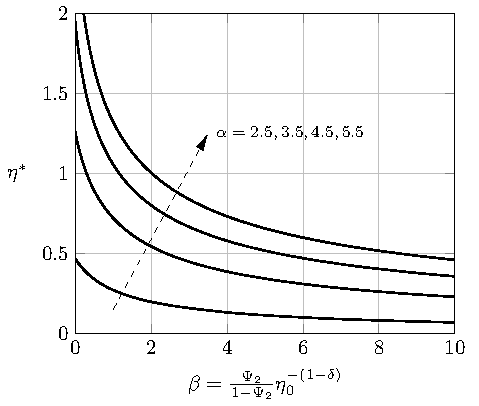
\includegraphics[]{./Figures/Ch7_optimum_partition.pdf}	
	\caption{Optimum spectral efficiency $\eta^*$ of the first class as a function of the parameter $\beta$, which is an increasing function of the parameter $\Psi_2$ of the second user class.}
	\label{fig:optimum_partition}
\end{figure}
Recall that $\beta$ is an increasing function of $\Psi_2$, which, in turn, is a comprehensive measure of the performance requirement of Class 2 users. As expected from the previous discussion, $\eta^*$ decreases as the performance requirement of the second class becomes more stringent, i.e., when $\Psi_2$ increases. This behavior of $\eta^*$ can be explained by recalling that higher spectral efficiency requires higher SIR threshold $\theta_1$, causing stronger interference to users of the second class.
%
This increased interference reduces the maximum admissible rate $a_2$ and increases the minimum achievable delay $D_2$. Since $\Psi_2$ is kept fixed in this optimization problem, $\eta^*$ must be limited. In fact, from Eq. \eqref{eq:theor01} we can see that if $\Psi_2$ increases, then $\Psi_1$ must be reduced in order to keep the system stable.
%
The propagation environment also affects the optimum spectrum efficiency. Environments with larger path loss exponent $\alpha$ reduce the interference among users, improving the channel quality and allowing for the use of higher spectral efficiency transmission schemes.

Finally, note that without the second user class ($\Psi_2 = 0$), we have $\beta=0$ and the equation for $\eta^*$ in Theorem~\ref{th:optimum_eta} has a closed form solution, which is
\begin{equation}\label{eq:opt_eff}
	\eta^*(\beta=0) = \tfrac{\alpha}{2} +
    W_0\big(-\tfrac{\alpha}{2}\,\euler^{-\alpha/2} \big),
\end{equation}
where $W_0$ is the principal branch of the Lambert-$W$ function, which is defined as the solution on $[-1,\infty)$ of the equation $W_0(x)\,\euler^{W_0(x)} = x$, for $x \ge -1/\euler$.
%
The above result is consistent with \cite[Theorem~2]{jindal2008bandwidth}, where the optimization is over the traffic density achievable and the system consists of a single user class. Expression \eqref{eq:opt_eff} was also obtained by Haenggi in \cite{Haenggi_Lambert}.

As discussed in \cite{jindal2008bandwidth}, the quantity $\delta \eta^*(0) \to 1$ as $\delta \to 0$ (i.e. $\alpha\to\infty$), which means that $\eta^*(0)$ grows asymptotically as $\alpha/2$ when the path loss exponent $\alpha$ tends to infinity.
%
However, for a given $\beta>0$, the same does not hold true. We can show that $\delta \eta^*(\beta) \to 0$ as $\delta \to 0$.

In fact, we can be more precise and show through \eqref{eq:Theor02} that if $\beta>0$, then $\sqrt{\delta} \eta^* \to 1/\sqrt{\beta}$ as $\delta\to 0$, which means that $\eta^*$ grows asymptotically as $\sqrt{\alpha/2\beta}$ when the path loss exponent $\alpha$ tends to infinity.
%
Thus, by introducing interference from another class in the system ($\beta>0$, i.e. $\Psi_2>0$), we change the asymptotic behavior of the optimal spectral efficiency from linear growth to squared root growth with respect to the path loss exponent $\alpha$.

This asymptotic result can be seen in Figure~\ref{fig:optimum_eta_delta}, where we plot the optimal spectral efficiency $\eta^*$ adjusted by the multiplicative factor $\sqrt{\beta\delta}$, which corresponds to the reciprocal of the asymptote as $\delta$ tends to $0$ (that is why all curves converge to $1$ at $\delta = 0$).
%
Another simple asymptote of $\eta^*$ is given by $2(1-\delta)/(1+\beta)$ when $\delta$ tends to $1$ (i.e. $\alpha\to2$).

\begin{figure}[!t]
	\centering
	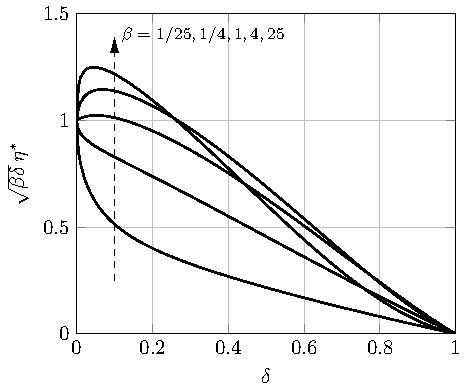
\includegraphics[]{./Figures/Ch7_optimum_eta_delta.pdf}	
	\caption{Optimum spectral efficiency $\eta^*$ of the first class adjusted by the multiplicative factor $\sqrt{\beta\delta}$ as a function of the parameter $\delta = 2/\alpha$ for several values of $\beta$.}
	\label{fig:optimum_eta_delta}
\end{figure}

Also, we can obtain a generalization of \eqref{eq:opt_eff} when the performance requirements of Class 2 is small (i.e., $\Psi_2 \approx 0$), which is equivalent to $\beta \approx 0$. Then, we have the following first order expansion for the optimum spectral efficiency
\begin{align} \label{eq:eta_expansion}
    \frac{\eta^*\!(\beta)}{\eta^*\!(0)} = 1 - \frac{(1-\delta)\eta^*\!(0)^{1-\delta}}{\eta^*\!(0)+1-\frac{1}{\delta}} \beta + \cal{O}(\beta^2),
\end{align}
as $\beta$ tends to zero, $\eta^*\!(0)$ is given by Eq.~\eqref{eq:opt_eff} and $\cal{O}$ is the big O notation as defined in Definition~\ref{def:landau}.
% \footnote{
% We say $f(x) = \cal{O}(g(x))$ as $x\to a$, if $\limsup\limits_{x\to a} \frac{|f(x)|}{g(x)} < \infty$.
% }.
%
The above expression is found using implicit differentiation on \eqref{eq:opt_eta} and some manipulations.

We can verify through \eqref{eq:eta_expansion} that the optimal spectral efficiency has a steeper (relative) decay for larger values of the path loss exponent $\alpha$, when $\alpha > 2.48$.
%
This means that the presence of interference from another class has a larger relative impact on the optimal spectral efficiency when $\alpha$ is large.

% \begin{figure}[!t]
% 	\centering
% 	\input{./Plots/optimum_partition_norm.tex}	
% 	\caption{Optimum spectral efficiency $\eta^*$ of the first class as a function of the parameter $\beta$, which is an increasing function of the parameter $\Psi_2$ of the second user class.}
% 	\label{fig:optimum_partition_norm}
% \end{figure}

% % % % % % % % % % % % % % % % % % % % % % % % % % % % % %
\subsection{Applications}
\label{sec:num}

In this section, we illustrate the analytical results through some numerical examples. Let the first and second user classes represent the opportunist and the main users of a given bandwidth $B_0$, respectively.
%
The opportunist users access the same frequency band as the main users and we perform bandwidth partitioning for the opportunistic access in order to improve the performance of the opportunist users for a given performance of the main users, which is equivalent to fixing the quantity $\Psi_2$.

From now on, we shall use the numerical values in Table~\ref{tab:user_classes} for the numerical examples.
%
\begin{table}[!ht]
    \centering
        \caption{Parameter values.}
    \begin{tabular}{ c|l }
    \hline
    Parameters & Values \\
    \hline\hline
     $\lambda_1$        & $\SI{0.005}{/m^2}$      \\
     $\lambda_2$        & $\SI{0.002}{/m^2}$      \\
     $\overline{R}_1$   & $\SI{10}{m}$            \\
     $\overline{R}_2$   & $\SI{20}{m}$           \\
     $\eta_0$           & $\SI{0.2}{bits/s/\hertz}$   \\
     $p_1=p_2$          & $1$   \\
    \hline
    \end{tabular}
    \label{tab:user_classes}
\end{table}
%
We begin our analysis by comparing the stability regions with and without bandwidth partition. 
% Let the system parameters be $\lambda_1 = \SI{0.005}{/m^2}$, $\lambda_2 = \SI{0.002}{/m^2}$, $\overline{R}_1 = \SI{10}{m}$, $\overline{R}_2 = \SI{20}{m}$ and the (initial) spectral efficiency $\eta_0 = 0.2\,\ln(2)\,\si{nats/s/\hertz}$ for both classes.
%
Our approach to determine the stability regions is the following: we begin by using  Theorem~\ref{th:optimum_eta} to find the optimum spectral efficiency $\eta^*$ of the first class for a given value of ${\Psi_2\in(0,1)}$ (see Remark~\ref{rmk:Th.Stb.}); then, we choose the number of sub-bands $M$ as the closest integer%
\footnote{This is a functional thumb rule to find the optimum number of partitions $M^*$. However, the ideal approach is to verify through the objective function if the best is to round up or round down.
In our plots, we used the thumb rule, since there is no visual difference.}
to $\eta^*/\eta_0$ (it is worth remembering that $\Psi_2$ is fixed, so the performance requirements of Class 2 are still satisfied); finally, we use Theorem~\ref{th:identity} along with the fact that $p_1=p_2=1$ maximizes the stability region to obtain the union of the stability regions for all the transmit power ratios $P_1/P_2$ and for all medium access probabilities $p_1$ and $p_2$. The results are shown in Fig.~\ref{fig:optimum_stab_region} for $\alpha = 2.5$ and $4.5$.
%
\begin{figure}[!t]
	\centering
	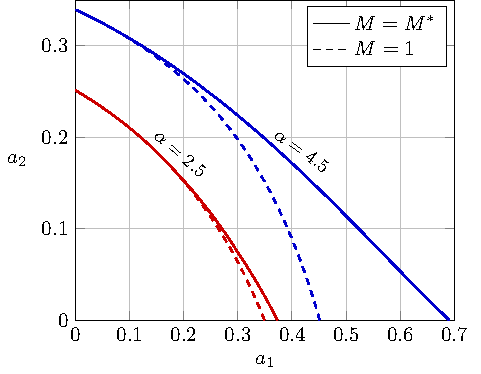
\includegraphics[]{./Figures/Ch7_optimum_stab_region.pdf}%
	\caption{Stability regions of the network for different values of path loss exponent $\alpha$. The arrival rates $a_1$ and $a_2$ are the opportunist and main users, respectively; full and dashed curves correspond to the boundaries of the stability region with and without bandwidth partition, respectively. Parameter values are shown in Table~\ref{tab:user_classes}.}
	\label{fig:optimum_stab_region}
\end{figure}
%
We can see that the optimization of the spectral efficiency of the first user class (through bandwidth partitioning) expands the stability region. Note that when the path loss exponent $\alpha$ is small (close to 2), the optimization does not improve significantly the system performance.
%
Another observation is that if the traffic from main users (Class 2) is high, i.e., it is responsible for the majority of the interference, then it makes practically no difference to perform bandwidth partitioning in the opportunist class (Class 1). On the other hand, as the traffic from opportunist users increases, the impact of the optimization also increases
% \textcolor{red}{(esse melhor desempenho no canto direito inferior da região ($a_1$ alto e $a_2$ baixo) tem a ver apenas com a baixa interferência causada pelos usuários 2? Acho que poderíamos explorar esse melhor desempenho nessa região, pois é a região de interesse da ideia da partição.)}.

Let us now consider another example to analyze the effects of bandwidth partitioning on the mean delay.
% For this, we set the initial spectral efficiency for the opportunist class $\eta_0 = 0.2\,\ln(2)\,\si{nats/s/\hertz}$, the access probabilities $p_1=p_2=1$.
%
We then determine the mean delay $D_1$ of the opportunist class as a function of its arrival rate of packets $a_1$, for $\Psi_2 = 0.25, \, 0.5, \, 0.75$. Note that $\Psi_2$ can be seen here as a measure of the performance required by the main class (see Remark~\ref{rmk:Th.Stb.}). The procedure to find $M^*$ is analogous to the one used in the last example. The results are shown in Fig.~\ref{fig:optimum_delay}.
%
\begin{figure}[!t]
	\centering
	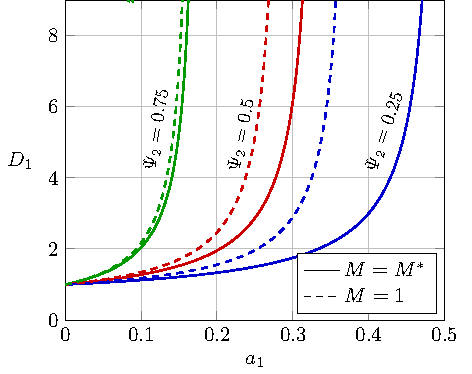
\includegraphics[]{./Figures/Ch7_optimum_delay.pdf}%
	\caption{Opportunist (first class) mean delay $D_1$ as a function of opportunist arrival rate $a_1$, for different values of the main user performance requirement $\Psi_2$. Full and dashed curves correspond to the cases with and without bandwidth partition, respectively. Parameter values are shown in Table~\ref{tab:user_classes}.}
	\label{fig:optimum_delay}
\end{figure}
%
When the performance requirements of the main users are modest (small $\Psi_2$), bandwidth partitioning allows for a more efficient use of the channel by opportunist users, i.e., a larger arrival rate $a_1$ is possible, or a smaller mean delay is achieved. On the other hand, and as expected from the previous analysis, we can also see that when the requirements of main users become more stringent (larger $\Psi_2$), then less noticeable is the improvement from the bandwidth partitioning.
%
\begin{figure}[!t]
	\centering
	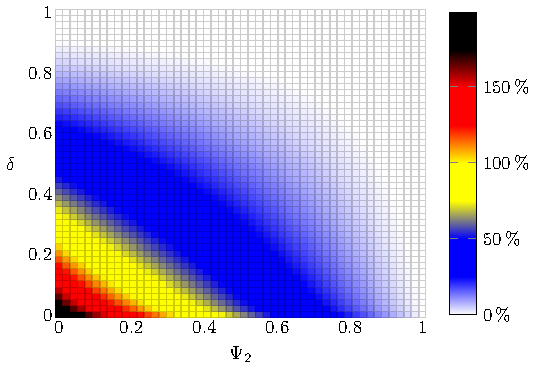
\includegraphics[width=0.7\columnwidth]{./Figures/Ch7_a_ratio.pdf}%
	\caption{Maximum throughput relative improvement of Class 1 after band partition. Parameter values are shown in Table~\ref{tab:user_classes}.}
	\label{fig:a_ratio}
\end{figure}

% \begin{figure}[!t]
% 	\centering
% 	\input{./Plots/a_ratio_v2.tex}	
% 	\caption{Maximum throughput improvement of Class 1 after band partition. Parameter values are shown in Table~\ref{tab:user_classes}. \textcolor{red}{Daria para colocar ``curvas de nível'', relativas a alguns valores de ganho?}}
% 	\label{fig:a_ratio_v2}
% \end{figure}

Figure~\ref{fig:a_ratio} shows the relative improvement of the maximum throughput after band partition of Class 1 relative to the maximum throughput before band partition, for all possible values of $\Psi_2$ and $\delta$. For example, in the yellow region, we have almost doubled the throughput ($\approx 100\%$ improvement) after implementing the optimum number of band partitions. As we have previously seen through figures \ref{fig:optimum_stab_region} and \ref{fig:optimum_delay}, the bandwidth partitioning strategy of the first user class improves significantly the performance of Class 1 users as the Class 2 performance requirements $\Psi_2$ is small and the path loss exponent $\alpha$ is large (which is equivalent to small $\delta = 2/\alpha$). On the other hand, when the path loss exponent $\alpha$ is small or the performance requirements of the main (Class 2) users $\Psi_2$ is stringent, there is almost no gain in performing bandwidth partitioning of the opportunistic class (Class 1).

% % % % % % % % % % % % % % 
\section{Summary} \label{sec:summ_P2_03}

In this chapter, we derived necessary and sufficient conditions for stability in a network with $N$ user classes; we also provided simple closed form expressions for the packet success probability and mean delay. The advantage of using this model as a base to model other network effects is its analytic tractability.
%
As an example, we were able to derive simple conditions to verify the stability of an interference-limited network with undetermined transmit powers using Corollary~\ref{cor:stab}.
%
We also solved (analytically and in closed form) two optimization problems regarding the minimization of the delays in a network and maximization of the total throughput per unit of area.
%
An interesting insight from the optimization problems is that the best solution to maximize the throughput of a channel is not necessarily using solely the user class with the best link quality, i.e., a mix with other user classes may result in better use of the channel.
% 
% All in all, this paper provides a simple way to evaluate the existing trade-offs involved in the design of wireless networks when different classes of nodes co-exist.

Further, we showed that, under certain conditions, bandwidth partitioning can significantly improve the performance of the network (under stability condition) by means of higher allowable arrival rates or lower mean delays. This is the first time the problem of bandwidth partitioning is treated analytically for two interacting user classes, for which arriving packets are queued.